\documentclass[12pt,a4paper,twoside]{report}

\usepackage[a4paper,left=2.5cm,right=2.5cm,top=2.5cm,bottom=2.5cm]{geometry}
\usepackage{fontspec}
\setmainfont{Arial}
\usepackage{setspace}

\usepackage{booktabs, multirow, array}


%%IMPORTED PACKAGES
\usepackage{amsmath}
\usepackage{amssymb}

\onehalfspacing
\setlength{\parindent}{0pt}
\pagenumbering{gobble}

\begin{document}

% Page 1: blank
\cleardoublepage\null\newpage

% Page 2: blank
\null\newpage

% Page 3: dedication / acknowledgements / blank
\begin{center}
% Dedication or acknowledgements here
\end{center}
\newpage

% Page 4: blank
\null\newpage

% Thesis starts on right-hand odd page
\cleardoublepage
\pagenumbering{arabic}

\tableofcontents
\cleardoublepage

\chapter{Introduction}

Humans have always shown an intense desire to understand and replicate nature’s mechanisms. The barter and the merchants, were the foundation of how our knowledge and
goods were exchanged across all the known world. With time, and the continuous pursuit
of understanding, man were able to create a global mean of exchange and interaction:
financial markets. These markets are not merely economic engines, that fuels our nations
with much needed resources, but complex systems where governments, economic actors,
and investors associate value to limited resources. The study of these systems lies at
the heart of Quantitative Finance, a discipline that builds on the premise that market
dynamics can be comprehend through mathematical and statistical frameworks.\\

However, modeling financial assets remains a central challenge in today’s world, since
such data are characterized by complex stochastic dynamics that frequently break the
assumptions of normality and stationarity. Indeed, these time series frequently exhibit
”stylized facts” \cite{cont2001empirical}, or known empirical regularities such as volatility clustering, heavy-tailed
return distributions, leverage effects, and sudden, discontinuous jumps. Modeling these
non-linear, high-dimensional has proven complicated. Nevertheless, with the increase of complexity within financial markets, the need for synthetic data as a source of information for scenario analysis, backtesting, stress test, and data augmentation has soared.\\

Traditionally, academics have relied on statistical tools like ARIMA \cite{box1970time} for trend analysis
and GARCH \cite{bollerslev1986generalized} for modeling heteroskedasticity. Instead, in the continuous-time domain,
the Geometric Brownian Motion (GBM) has shown to be a foundational building block
for asset price modeling and, particularly, for derivative pricing through Monte Carlo
methods. While these models often offer high interpretability and computational efficiency, they often lack the expressivity to capture the complex distribution of financial
time series.\\

With the raise of Machine Learning and later Deep Learning new opportunities came.
Two framework, in particular, were promising: Generative Adversarial Networks (GANs) \cite{goodfellow2014generative, creswell2018generative}
and Variational Autoencoders (VAEs) \cite{kingma2014auto, kingma2019introduction}. While both proved exceptional in various domains, they are bound by some core limitations, GANs are notoriously unstable to train and prone to mode collapse, while VAEs produce overly smoothed samples and suffer
from posterior collapse, therefore failing to provide the same level of expressivity seen
in GANs. In the meantime a diverse set of architectures and functionalities has been
explored, including Energy-Based Models \cite{lecun2006tutorial}, Normalizing Flows \cite{rezende2015variational}, and lastly Diffusion Models \cite{ho2020ddpm, song2021score, song2021denoising, rombach2022high, dhariwal2021diffusion}. These are now the primary choice in many fields, because they effectively combine
expressivity with training stability and indeed they are the state-of-the-art for image and video generation. Interestingly, while the financial sector has seen a surge in Large Language Models (LLMs)
for natural language tasks such as sentiment analysis, classification task, and back-end
automation, the application of generative diffusion models to financial time series is still limited.\\

To address the gap, this work proposes to combine the Conditional Score-based Diffusion Model for Imputation (CSDI) \cite{tashiro2021csdi} into the Elucidated Diffusion Model (EDM) \cite{karras2022elucidating}
framework. The previous fusion is natural, since CSDI utilize a Transformer architecture, which was originally
designed to capture temporal and feature dependencies for imputation, while EDM defines a clear and malleable design environment for diffusion models.\\

The research is structured in two sequential phases. \textbf{Phase~1} replicates the work of Kim et al.\ \cite{kim2025diffusion}, implementing their VE-, VP-, and GBM-inspired SDE variants on univariate Close log-returns, in order to establish a validated baseline and expose the design ambiguities present in the original paper. \textbf{Phase~2} then extends this foundation by embedding a CSDI backbone within the EDM framework and introducing multivariate conditioning: the model learns to generate Close log-returns given the contemporaneous Open, High, and Low observations. This sequential structure is deliberate --- replication first ensures that any performance difference observed in Phase~2 can be attributed to the novel design choices rather than to implementation artefacts.\\

The research questions addressed in the two phases are therefore distinct:

\textbf{Phase 1 \textemdash{} Replication}
\begin{itemize}
    \item Are CSDI-based architectures able to learn the stylized facts of financial time series?
\end{itemize}

\textbf{Phase 2 \textemdash{} EDM-CSDI}
\begin{itemize}
    \item How do EDM design choices help in elucidating learning behaviors?
    \item Does the introduction of conditioning information aid in improving the model's performance?
\end{itemize}

In asnwering the previous question, the following contributions were achieved:
\begin{itemize}
    \item Framework integration: we adapt the CSDI architecture within the EDM to ensure mathematical clarity, replicability, and effective control over the reverse diffusion process for financial data.
    \item Comprehensive evaluation: we test the model both on synthetic datasets and realworld observations, employing evaluation measures that include finance-specific metrics and statistical ones.
    \item Stylized fact assessment: we evaluate the model’s ability to reproduce the core stylized facts of financial markets, specifically heavy tails, volatility clustering and leverage effects, often neglected in other generative models.
\end{itemize}

In conclusion, this thesis contributes to the exploration of diffusion models for financial time series, empirically validating the results and generalizing the design framework to enable easier replicability and a higher degree of control over training choices.
This work commences with a literature review covering financial time series modeling from classical methods to deep learning ones, and the specifics of EDM and CSDI implementations. Subsequently, the theoretical framework is presented, discussing stochastic differential equations and the mathematical foundations of diffusion models. Next, the architectural and training settings are described, detailing how EDM fits within this picture. Chapters~\ref{ch:data_setup} and~\ref{ch:evaluation_methodology} cover data preprocessing and evaluation metrics shared across both phases; the experiments chapter then presents results organized sequentially, Phase~1 first and Phase~2 second. The thesis closes with a discussion of limitations and directions for future work.

The two phases differ along four structural dimensions: problem setup, diffusion process, training objective, and sampling strategy. Tab.~\ref{tab:comparisons} provides a compact side-by-side reference for these differences; the reader is encouraged to return to it while navigating the technical chapters.
% Required packages: booktabs, multirow, array
% \usepackage{booktabs, multirow, array}
\begin{table}[htbp]
\label{tab:comparisons}
\centering
\footnotesize
\renewcommand{\arraystretch}{1.35}
\setlength{\tabcolsep}{5pt}
\begin{tabular}{
  >{\itshape}p{2.0cm}
  p{3.3cm}
  p{4.65cm}
  p{4.65cm}
}
\toprule
\normalfont\textbf{Category}
  & \textbf{Dimension}
  & \textbf{Phase 1 \textemdash{} Replication}
  & \textbf{Phase 2 \textemdash{} EDM-CSDI} \\
\midrule
%--- Problem setup ---------------------------------------------------
\multirow{4}{2.0cm}{Problem setup}
  & Primary objective
  & Replicate Kim et al.\cite{kim2025diffusion}; validate VE, VP, and GBM-inspired
    variants on unconditional univariate generation
  & Conditional generation of Close log-returns given observed O, H, L;
    CSDI backbone integrated within the EDM framework \\[3pt]
  & Channels $K$
  & $K=1$ (univariate close log-returns)
  & $K=4$ (OHLC; all channels as log-returns relative to $C_{t-1}$) \\[3pt]
  & Conditioning / masking
  & Unconditional: $m^{co}=0$; loss computed on all
    entries, no side information
  & \texttt{predict\_close}: $\{O,H,L\}$ fully observed, $\{C\}$ fully
    masked; fixed deterministic split \\[3pt]
  & Sequence length / stride
  & $L=2048$,\; $s=400$
  & $L=512$,\; $s=100$ \\
\midrule
%--- Diffusion process -----------------------------------------------
\multirow{4}{2.0cm}{Diffusion process}
  & Forward SDE family
  & VE; VP;
    GBM-inspired VE in log-price space
  & VE-style forward process within EDM preconditioning\\[3pt]
  & $\sigma_{data}$
  & Implicit; absorbed into the choice of $\sigma_{\max}$/$\sigma_{\min}$
  & $\sigma_{data}=1.0$ by construction
    (per-channel $z$-score normalisation) \\[3pt]
  & Noise schedule parameters
  & VE: $\sigma_{\max}{=}1,\;\sigma_{\min}{=}0.01$;\;
    GBM: $\sigma_{\max}{=}10,\;\sigma_{\min}{=}0.1$;\;
    VP: $\beta_{\max}{=}8,\;\beta_{\min}{=}0.01$
  & $P_{mean}{=}{-1.4}$,\;$P_{std}{=}1.8$
    (ablation-tuned) \\[3pt]
  & Noise level sampling
  & $t\sim\mathcal{U}[0,1]$
  & $\ln\sigma\sim\mathcal{N}(P_{mean},P_{std}^{2})$;\\
\midrule
%--- Training objective ----------------------------------------------
\multirow{5}{2.0cm}{Training objective}
  & Prediction target
  & Noise $\boldsymbol{\epsilon}$ (DSM)
  & Clean data $x_{0}$ (MMSE) \\[3pt]
  & Loss function
  & $\mathbb{E}\!\left[
      \|\boldsymbol{\epsilon}
        - \boldsymbol{\epsilon}_{\theta}(x_{t},t)
      \|^{2}_{m^{ta}}
    \right]$
  & $\mathbb{E}\!\left[
      \lambda(\sigma)
      \|D_{\theta}(x_{t};\sigma)-x_{0}
      \|^{2}_{m^{ta}}
    \right]$ \\[3pt]
  & Loss weighting $\lambda$
  & $\lambda(\sigma_{i})=\sigma_{i}^{2}$\;
  & $\lambda(\sigma)=c_{out}(\sigma)^{-2}$\;\\[3pt]
  & Preconditioning
  & None; raw network $F_{\theta}(x_{t};\,t)$
  & $D_{\theta}=c_{skip}\,x
      +c_{out}\,F_{\theta}(c_{in}\,x;\,
      c_{noise})$,\; with $\sigma_{data}{=}1.0$ \\[3pt]
  & Diffusion-step embedding
  & Discrete step index $t$
    (sinusoidal basis $+$ two linear layers with SiLU)
  & $c_{noise}(\sigma)=\tfrac{1}{4}\ln\sigma$;
    compresses the dynamic range of $\sigma$ to a bounded scalar \\
\midrule
%--- Sampling --------------------------------------------------------
\multirow{2}{2.0cm}{Sampling}
  & Numerical sampler
  & Euler--Maruyama and probability flow ODE
  & Heun second-order predictor--corrector on the probability flow ODE\\[3pt]
  & Sampler--training coupling
  & Coupled
  & Decoupled \\
\bottomrule
\end{tabular}
\caption{Design differences between Phase~1 (replication of Kim et al., 2025) and
Phase~2 (EDM-CSDI).}
\end{table}

%Chapter 2, look at chapter2.tex
\chapter{Background and Related Work}
\label{ch:literature_review}
\section{Financial Time Series and Stylized Facts}
\label{sec:fts_literature}
In order to understand the methodology, it is important to define what a financial time series (FTS) is and which statistical challenges do their modeling pose.

One of the core focus of FTS analysis are log-returns, expressed as:
\begin{equation}
    \label{eq:log_returns}
    r_t=\log\left(\frac{C_t}{C_{t-1}}\right)
\end{equation}
where $C_t$ is the closing price on any given day $t$. Alongside this, it is useful to consider opening price $\left(O_t\right)$, highest price $\left(H_t\right)$, and lowest price $\left(L_t\right)$, for brevity OHLC values. 

It is standard in the literature to consider \textit{adjusted} versions of prices, where given a nominal price $S_t$, the adjusted price is $\widetilde{S}=A_tS_t$.
Adjustments correct for mechanical price changes caused by corporate actions, such as stock split, dividends payments, and others. This is done in order to retain comparability over time. For instance, a 2-for-1 stock split, cause the stock price to be divided by two, while each investor's total economic holding remains unchanged. Without adjustment, this artificial price drop would appear as a large negative return. These adjustments are cumulative. 

FTS log-returns exhibit four core characteristics:
\begin{itemize}
    \item Not Gaussian IID: returns do not follow a random walk.
    \item Fat Tails: returns distribution decay according to the power law, $P(|r|>x)\sim x^{-\alpha}$, with the typical exponent $\alpha\in[3,5]$ for many class of assets.
    \item Volatility Clustering: autocorrelation of absolute returns, $|r_t|$, and square returns, \(r^2_t\), decays hyperbolically, respecting \(\operatorname{Corr}(|r_t|, |r_{t+k}|)\sim k^{-\beta} \quad \beta\in [0.1,0.5]\).
    \item Leverage Effect: negative returns are followed by higher future volatility asymmetrically \cite{black1976studies}. This is measure through lead-lag correlation \(L(k)=\mathbb{E}\left[r_tr_{t+k}^2 \right]/\mathbb{E}\left[r_t^2\right]^2<0\).
\end{itemize}

\begin{figure}[htbp]
    \centering

    \begin{subfigure}{0.32\textwidth}
        \centering
        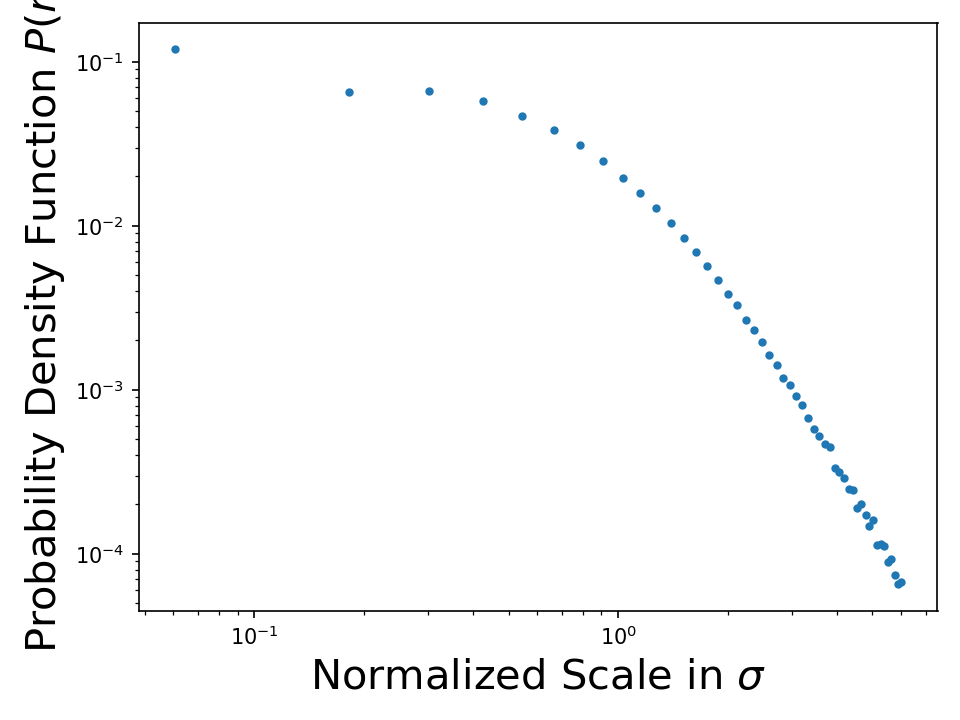
\includegraphics[width=\linewidth]{images/gen_dist_replication_returns_other_pos_log.png}
        \caption{Heavy-tail distribution}
        \label{fig:ref_distribution}
    \end{subfigure}
    \hfill
    \begin{subfigure}{0.32\textwidth}
        \centering
        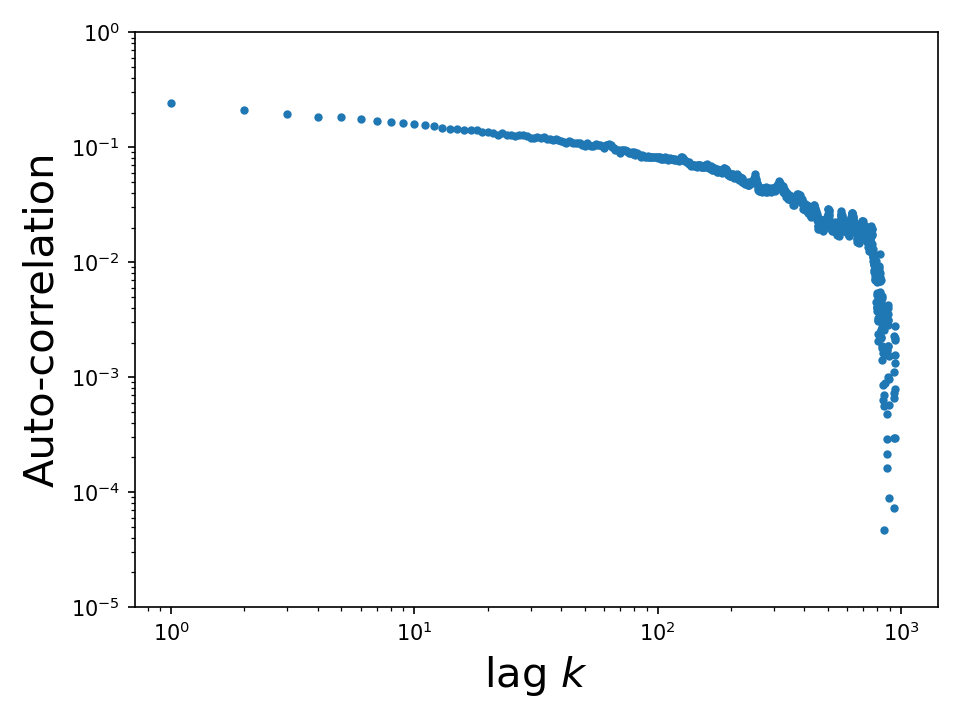
\includegraphics[width=\linewidth]{images/ref_vol_clus_replication_returns_other.png}
        \caption{Volatility clustering}
        \label{fig:ref_vol_clustering}
    \end{subfigure}
    \hfill
    \begin{subfigure}{0.32\textwidth}
        \centering
        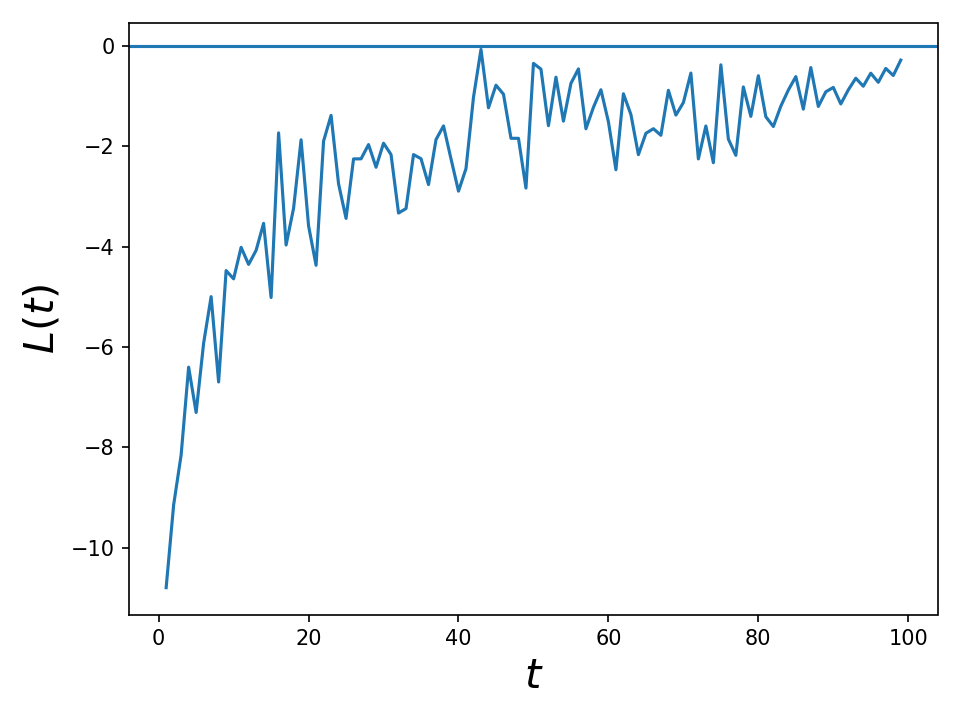
\includegraphics[width=\linewidth]{images/lev_eff_replication_returns_other.png}
        \caption{Leverage effect}
        \label{fig:ref_lev_eff}
    \end{subfigure}

    \caption{Stylized Facts for FTS, S\&P500 log-returns.}
    \label{fig:three_graphs}
\end{figure}

It is important to state that financial returns do not follow a Gaussian behavior, indeed large price fluctuations occur more frequently than under Brownian motion, breaking random walk assumption \cite{mandelbrot1963variation, fama1965random}. Moreover, the fact that returns have polynomial-like tail decay \cite{cont2001empirical} implies that, contrary to what was believed before \cite{mandelbrot1963variation}, they have finite variance, and often unstable of infinite fourth moment \cite{gopikrishnan1999scaling}. Therefore, it is modern consensus that returns are not necessarily symmetric Lévy-stable process \cite{mantegna1995scaling}, but that assuming a Gaussian tail distribution would significantly underestimate risk. 

\section{Classical Models}
\label{sec:classical_models_literature}
Classical FTS models often address the non-Gaussian behavior by extending upon the basic Brownian motion framework because of its favourable framework. In particular, GARCH-like models \cite{bollerslev1986generalized} focus on time-varying volatility, where by construction the model is conditionally heteroskedastic, meaning that large shocks are followed by higher volatility and period of calm by lower ones. Merton's jump diffusion \cite{merton1976option} instead build on the continuous Geometric Brownian Motion (GBM) by adding a Poisson jump component, the jumps. These are two common model to capture stylized facts about financial data, which is why they would work as baseline. 

In a GARCH(1,1) we have that the conditional variance behaves accordingly to:\(\sigma_t^2=\omega+\alpha\epsilon_{t-1}^2+\beta \sigma_{t-1}^2\), where \(\omega>0\) and \(\alpha, \beta \ge 0\), with a persistent condition \(\alpha+\beta<1\). Despite their parsimony, GARCH models remain a competitive benchmark in financial time-series modelling due to their interpretability, tractable likelihood, and well-known statistical properties. 

In order to understand Merton's model we have to introduce first the GBM. Given an asset price \(S_t\) it is said to follow a GBM if:
\begin{equation}
    \label{eq:blackscholes}
    dS_t=\mu S_td\tau+\nu S_tdW_t
\end{equation}
where \(\mu\) is the constant drift, \(\nu>0\) is the constant volatility, and \(W_t\) is a standard Brownian motion. The core feature of this process is the multiplicative structure of the noise term, which is scaled by price level. Applying Itô's Lemma to \(\log S_t\) it is possible to derive:
$$S_t=S_0\exp{\left[\left(\mu-\frac12\nu^2\right)\tau+\nu W_t\right]}$$
therefore with the GBM assumption, , Black and Scholes \cite{black1973pricing}, implied that log-returns are normally distributed over any interval, while heteroskedasticity is introduced in price space. Their model remain highly influencial even nowadays, nevertheless it has some fundamental limitations due to the inability of Gaussian's innovations to replicate the heavy tails, excess kurtosis, and sudden discontinuities exhibited by real returns. 

Merton addressed this by imposing a compounded Poisson jump process onto the GBM \cite{merton1976option}, yielding the model that takes his name:
$$dS_t=\mu S_tdt+\nu S_tdW_t+S_{t^-}(J-1)dP_t$$
where \(P_t\) is the Poisson process with intensity \(\lambda\) and J is a random jump multiplier \(J\sim \mathcal{N}(\mu_j, \sigma_J^2)\). This result in log-returns distribution that is a Poisson's weighted mixture of Gaussians. 

Both of these models impose parametric distributions, while this enable easier interpretation and a well understood behavior that makes them valuable baselines, it is also their limiting factor, that do not enable them to learn complex, highly dimensional joint distribution, and is also why they require re-fitting whenever their estimation regime changes.

\section{Deep Generative Models}
Deep generative models are non-parametric, therefore they learn implicitly the data distribution, \(p_{\text{data}(x)}\), and can theoretically learn all the stylized facts simultaneously, including temporal and feature dependencies. Before diffusion models, two families of models mostly dominated the FTS modeling and generation scene: GANs \cite{goodfellow2014generative, creswell2018generative,yoon2019time,vuletic2024fingan} and VAEs \cite{kingma2014auto, kingma2019introduction}. GANs, Generative Adversarial Networks, consist of a non-cooperative minmax game between a Generator \(G_\theta(z)\) and a Discriminator \(D_\phi(x)\): by learning implicitly the distribution without explicit likelihood constraints they are able to avoid over-smoothing and generate more sharp and diverse samples. On the other hand, GANs often suffer of mode collapse, when the Generator fail to capture fully the target distribution \(p_{\text{data}(x)}\), mapping only to few modes. Moreover, GANs suffer from training instability due to the non-convex nature of the minmax problem, which makes the optimization difficult.

VAEs, Variational Autoencoders, provide a probabilistic framework where input data \(x\) are mapped into a latent space through an encoder and reconstructed via a decoder \(p_\theta(x|z)\), with the system trained to maximise the Evidence Lower Bound (ELBO), fundamentally balancing a reconstruction term and a KL regularisation term. While theoretically sounding, VAEs suffer mainly from two limitations: posterior collapse and over-smoothing. The former, happens when the KL regularisation term dominates early training phases and push the approximate posterior towards the prior before any informative encoding is learned, degenerating into an unconditional mean model. The latter, because of the Gaussian decoder assumption, minimise square reconstruction error, which sistematically compress variance and suppress tail events. Both model families have limitations that make them difficult to apply to FTS. In contrast, diffusion models provide a probabilistic framework and a stable training objective, at the cost of slower sampling.

\section{Score-based Diffusion Models}
\label{sec:scorediffmodels}
Score-based diffusion models revolve around a simple idea: rather than learning to generate data directly, a model could learn to denoise it. If data are gradually corrupted, up to a point, where they become indistinguishable from a fixed prior, the generation is then reduced to learn how to reverse the corruption process, one step at the time. What makes the reversal possible is the score function,\(\nabla_x \log p(x)\), that intuitively points in the direction one should move a noisy sample to make it more likely under the current data distribution.

The score function is chosen to represent the probability distribution of the generative model, because it encodes the geometry of the distribution and it does not require the computation of the normalizing constant, $Z_\theta$, which are often complex and unstable. Therefore, our goal is to learn a function that can approximate the score, \(s_\theta(x)\approx\nabla_x \log p(x)\) by minimizing the Fisher divergence between \(\mathbb{E}_{p(x)}=\left[\|\nabla_x\log p(x)-s_\theta (x)\|^2_2\right]\) the two distributions. This can be achieved without knowing the ground truth through methods called score matching \cite{hyvarinen2005estimation, vincent2011connection}. 

Once we have trained a score-based model, we use Langevin dynamics \cite{parisi1981correlation} to draw samples from it. Due to the weighting of the Fisher Divergence the score estimate are only reliable in high density region, but Langevin dynamics must traverse low-density regions to move between modes, guided by the score. To address this, data are perturbated with a sequence of noise levels, \(\sigma_1< \sigma_2< \dots<\sigma_L\), that populate low-density regions and makes score estimation accurate everywhere. Therefore, we move to estimating a Noise-Conditional Score-based Network (NCSN) \cite{song2019generative}, \(s_\theta(x,i)\), where \(i=1,2,\dots,L\). The choosen noise is often Gaussian \(\mathcal{N}(0,\sigma_i^2I)\) and the sampling is performed through annealed Langevin dynamics. This model is often referred to as Score Matching with Langevin Dynamics (SMLD). 

Independently, DDPM's authors \cite{ho2020ddpm} reached a similar framework, where the forward process is not motivated through score estimation, but is a fixed Markov chain that gradually injects Gaussian noise into the data. With the advantage that the marginal distribution at any step \(t\) has a closed form:
$$q(x_t|x_{t-1})=\mathcal{N}\left(x_t;\sqrt{1-\beta_t}x_{t-1}, \beta_tI\right), \quad q(x_t|x_0)=\mathcal{N}\left(x_t;\sqrt{\bar{\alpha}}x_0, (1-\bar{\alpha})I\right)$$
where \(\alpha_t:=1-\beta_t\) and \(\bar{\alpha}_t:=\prod_{s=1}^t\alpha_t\) \cite{ho2020ddpm}. They also shows that by reparametrizing \(x_t(x_0,\epsilon)=\sqrt{\bar{\alpha_t}}x_0+\sqrt{1-\bar{\alpha_t}}\epsilon\), where \(\epsilon \sim \mathcal{N}(0,I)\), the objective function get simpliefied to a noise prediction loss:
\begin{equation}
\label{eq:ddpm_noise_loss}
\mathcal{L}=\mathbb{E}_{t,x_0,\epsilon}\left[\|\epsilon -\epsilon_\theta(\sqrt{\bar{\alpha_t}}x_0+\sqrt{1-\bar{\alpha_t}}\epsilon,t)\|\right]  
\end{equation}

The key connection that makes the score matching tractable is due to Vincent \cite{vincent2011connection}, who showed that the intractable Fisher Divergence over the clean distribution \(p(x)\) can be replaced by a noisy one \(q_\sigma(\tilde{x}|x)=\mathcal{N}\left(\tilde{x};x,\sigma^2I\right)\), yielding Denoising Score Matching (DSM) objective:
$$\mathcal{L}_{\text{DSM}}=\mathbb{E}_{x\sim p(x),\space \tilde{x}\sim q_\sigma(\tilde{x}|x)}\left[\|s_\theta(\tilde{x},\sigma)-\nabla_{\tilde{x}} \log q_\sigma(\tilde{x}|x)\| \right]$$Since \(q_\sigma(\tilde{x}|x)\) is Gaussian then it is fully tractable with \(\nabla_{\tilde{x}} \log q_\sigma(\tilde{x}|x)=-\epsilon/\sigma\), where \(\tilde{x}=x+\sigma\epsilon\) and \(\epsilon\sim\mathcal{N}(0,I)\) is the added noise. The score therefore points from the corrupted sample \(\tilde{x}\) back towards the clean data \(x\), scaled by \(\sigma^2\). This reveals that the DDPM noise-prediction objective (Eq.\ref{eq:ddpm_noise_loss}) 
is not conceptually different from score matching up to a scaling factor, since 
$\epsilon_\theta(x_t,t)\approx -\sqrt{1-\bar{\alpha_t}}s_\theta(x_t,t)$. By 
consequence, DDPM and NCSN can be understood as discrete instantiations of a more 
general principle: corrupting data with a noise process and learning to reverse it 
by estimating scores. When training over multiple noise levels, the DSM objective 
becomes a weighted sum:
$$
\mathcal{L}_{\text{NCSN}} = \sum_{i=1}^{L} \lambda(\sigma_i)\,
\mathbb{E}_{x\sim p(x),\,\tilde{x}\sim q_{\sigma_i}(\tilde{x}|x)}
\left[\left\|s_\theta(\tilde{x}, \sigma_i) - 
\nabla_{\tilde{x}}\log q_{\sigma_i}(\tilde{x}|x)\right\|^2\right]
$$
Since the score satisfies $\nabla_{\tilde{x}}\log q_{\sigma_i}(\tilde{x}|x) = 
-\epsilon/\sigma_i$, its magnitude varies strongly across noise levels, and the 
choice of weighting $\lambda(\sigma_i)$ is non-trivial. Song \cite{song2019generative} 
proposes $\lambda(\sigma_i) = \sigma_i^2$ to approximately equalise the contribution 
of each noise level, but this choice is heuristic rather than principled. 

% Song score funcitions
% Song score functions
\begin{figure}[htbp]
  \centering
  {\small
  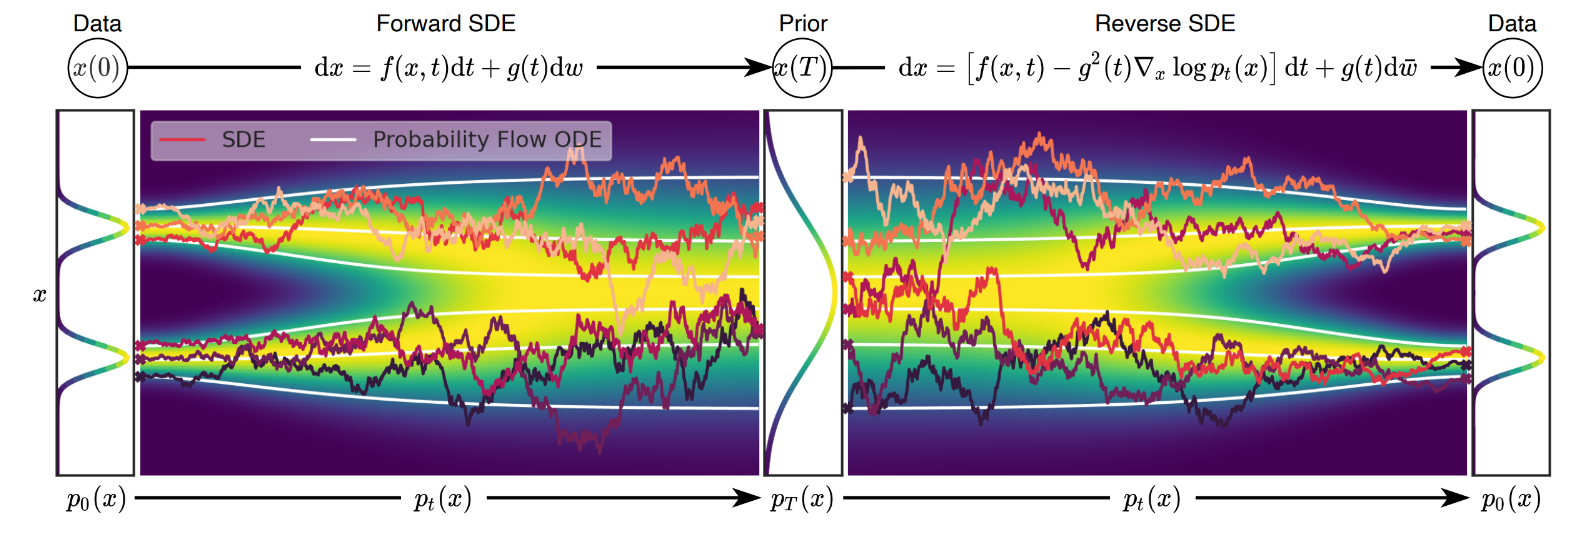
\includegraphics[width=\textwidth]{images/Overview_score_generative-modeling_Song.png}
  }
  \caption{Data can be mapped to a noise distribution (the prior) with an SDE (Eq.~\ref{eq:generalsde}), and reverse this SDE for generative modeling
(Eq.~\ref{eq:reverse_sde}). We can also reverse the associated probability flow ODE (Eq.~\ref{eq:probability_flow}), which yields a deterministic process that samples from the same distribution as the SDE. Both the reverse-time SDE and probability flow ODE can be obtained by estimating the score \(\nabla_x\log p_t(x_t)\). Source: Song et al.\ \cite{song2021score}.}
  \label{fig:sde_diffusion_process}
\end{figure}


Song \cite{song2021score} formalize the difusion model process by lifting DDPM and SMLD into a contiunous framework. He showed that the diffusion process \(\{x_t\}_{t=0}^T\) indexed by a continuous time variable \(t\in[0,T]\), where \(x_0\sim p_0\) is composed by i.i.d. samples of the dataset, and \(x_T\sim p_T\), for which we have a tractable form, can be modeled as the solution to an Itô SDE:
\begin{equation}
    \label{eq:generalsde}
    dx_t=f(x_t,t)dt+g(t)dW_t
\end{equation}
where \(W\) is the standard Wiener process, \(f(\cdot,t):\mathbb{R}^d\xrightarrow[]{}\mathbb{R}^d\) is a vector valued function called the drift coefficient of \(x_t\), and \(g(\cdot):\mathbb{R}\xrightarrow[]{}\mathbb{R}\) is a scalar function known as
the diffusion coefficient of \(x_t\). The SDE admits a unique strong solution provided the coefficients are globally Lipschitz \cite{oksendal2003stochastic}, and \(p_T\) is chosen to be a tractable prior, typically a Gaussian with fixed mean and variance, that contains no information about \(p_0\). 

The key insight is that the forward process admits a corresponding reverse-time SDE, in particular it has been shown \cite{anderson1982reversetime} that the reverse of a diffusion process is a diffusion process itself. By starting from samples \(x_T \sim p_T\) and reversing the process from \(t=T\) to \(t=0\), we can obtain samples \(x_0\sim p_0\) according to the relationship:
\begin{equation}
    \label{eq:reverse_sde}
    dx_t=\left[f(x_t, t)-g(t)^2\nabla_x\log p_t(x_t)\right]dt + g(t)d\bar{W}_t
\end{equation}

where \(\bar{W_t}\) is a standard Wiener process that flows back from \(T\) to \(0\). Since \(\nabla_x\log p_t(x_t)\) is unknown then we estimate it by using \(s_\theta(x_t,t)\). Importantly, Song et al. \cite{song2021score} showed that for any SDE (Eq.\ref{eq:generalsde}) there exists a corresponding deterministic Ordinary Differential Equation (ODE), called probability flow ODE, that produce the same family of marginal distributions \(\{p_t\}_{t\in[0,T]}\):
\begin{equation}
    \label{eq:probability_flow}
    dx_t=\left[f(x_t,t)-\frac12g(t)^2\nabla_x\log p_t(x_t)\right]dt
\end{equation}
substituting the intractable score with the learned one yields a Neural ODE, where given starting conditions $x_T\sim p_T$ we can deterministically sample to produce a sample from, approximately, \(p_0\). This sampling technique is possibly more efficient. 

Two specific SDE formulation that matched the SMLD and DDPM ones, in continuous time, hence when we assume that the number of noise steps \(N\xrightarrow[]{}\infty\), are: Variance Exploding (VE) and Variance Preserving (VP). The former sets \(f(\cdot,t)=0\) and is defined as:
\begin{equation}
    \label{eq:ve}
    dx_t=\sqrt{\frac{d[\sigma^2(t)]}{dt}}dW_t
\end{equation}
so that \(x_t=x_0+\sigma\epsilon\), where \(\epsilon\sim \mathcal{N}(0,I)\), therefore the marginal's variance grows unbounded as \(\sigma(t)\) increases. VP is instead:
$$dx_t=-\frac12 \beta(t)x_tdt+\sqrt{\beta(t)}dW_t$$
with drift \(f(x_t,t)=-\frac12\beta(t)x_t\) and \(g(t)=\sqrt{\beta(t)}\). This setting preserve unit variance when \(x_0\) has it as well with the marginal converging to \(\mathcal{N}(0,I)\) as \(t\xrightarrow[]{}T\).

The reverse SDE can be solved numerically through different samplers. 
Song \cite{song2021score} employs the Euler-Maruyama method, a first-order 
discretisation of the reverse-time SDE:
\begin{equation}
\label{eq:euler_maruyama}
x_{t+dt} \leftarrow x_t + \left[f(x_t,t) - g(t)^2 s_\theta(x_t,t)\right]|dt| 
+ g(t)\sqrt{|dt|}\,\epsilon, \quad \epsilon \sim \mathcal{N}(0,I)
\end{equation}
though any suitable numerical solver can in principle be substituted.

This continuous formulation has the advantage of decoupling the noise schedule 
from the choice of sampler, admitting common schedules such as linear, 
exponential, and cosine. However, both DDPM \cite{ho2020ddpm} and the SDE-based 
framework of Song \cite{song2021score} require hundreds of Neural Function 
Evaluations (NFEs) to produce a single sample, and neither provides a principled 
answer to how noise levels should be chosen, nor how network inputs and outputs 
should be scaled.

\section{Elucidating the Design Space of Diffusion Models (EDM)}
\label{sec:edm_literature}
Karras et al.\ \cite{karras2022elucidating} identify that prior formulations, including 
DDPM and Song's SDEs, choose in a dependable way four conceptually distinct design choices: the noise schedule, the parametrisation of network inputs and outputs, the weighting 
of the loss across noise levels, and the numerical solver used at sampling time. 
EDM separates these into four independent components and optimises each 
separately.

\textbf{Preconditioning} \quad EDM parametrises the denoiser as:
\begin{equation}
    \label{eq:edm_denoiser}
    D_\theta(x;\sigma) = c_{\text{skip}}(\sigma)\,x + 
    c_{\text{out}}(\sigma)\,F_\theta\!\left(c_{\text{in}}(\sigma)\,x;\, 
    c_{\text{noise}}(\sigma)\right)
\end{equation}
where $F_\theta$ is the raw neural network and 
$c_{\text{skip}}, c_{\text{out}}, c_{\text{in}}, c_{\text{noise}}$ are scalar 
functions of $\sigma$ chosen so that the inputs to $F_\theta$ have unit variance, 
the training targets have unit variance, and errors in $F_\theta$ are amplified as 
little as possible. For data with standard deviation $\sigma_{\text{data}}$, 
EDM sets:
$$
c_{\text{skip}}(\sigma)= \frac{\sigma_{\text{data}}^2}{\sigma^2 + 
    \sigma_{\text{data}}^2}, \quad 
    c_{\text{out}}(\sigma)= \frac{\sigma \cdot \sigma_{\text{data}}}
    {\sqrt{\sigma^2 + \sigma_{\text{data}}^2}}
$$
$$
c_{\text{in}}(\sigma)=\frac{1}{\sqrt{\sigma^2 + 
    \sigma_{\text{data}}^2}}, \quad
    c_{\text{noise}}(\sigma)=\frac{1}{4}\ln(\sigma)
$$
The skip connection $c_{\text{skip}}(\sigma)$ has a simpler interpretation: at low $\sigma$, $c_{\text{skip}} \to 1$ and the network mostly 
copies the input, a sensible prior when the noisy observation is already close to 
the data; at high $\sigma$, $c_{\text{skip}} \to 0$ and the network must 
reconstruct the clean signal from scratch. This mechanism helps stabilizing the training 
across the full noise range without requiring separate tuning for each noise level. 

\textbf{Loss weighting} \quad The EDM training objective is defined with respect to the denoiser 
$D_\theta(x;\sigma)$. Given a clean sample $x_0 \sim p_0$ and noise 
$\epsilon \sim \mathcal{N}(0, I)$, the noisy observation is 
$\tilde{x} = x_0 + \sigma\epsilon$, as in VE, and the loss is:
\begin{equation}
    \label{eq:edm_loss}
    \mathcal{L}_{\text{EDM}} = \mathbb{E}_{\sigma,\, x_0,\, \epsilon}
    \left[\lambda(\sigma)\,\left\|D_\theta(x_0 + \sigma\epsilon;\,\sigma) - 
    x_0\right\|^2\right]
\end{equation}
The effective weight for each sample on the raw network prediction $F_\theta$ is 
$\lambda(\sigma)\,c_{\text{out}}(\sigma)^2$. EDM sets 
$\lambda(\sigma) = c_{\text{out}}(\sigma)^{-2}$, which cancels out this factor and equalises loss contribution across all noise levels. Without this correction, high-noise steps would dominate the gradient signal, producing a model that denoises well at large $\sigma$ but fails to recover fine 
structure poorly, which is precisely the failure mode left unaddressed by NCSN. 

\textbf{Noise distribution} Rather than sampling $\sigma$ uniformly in $t$ as in DDPM, EDM concentrates training effort on the noise range that is most informative. At very low $\sigma$ the noisy input is nearly identical to the clean data, and at very 
high $\sigma$ the target collapses to the dataset mean. The informative region is in the middle, therefore EDM targets it by drawing:
\begin{equation}
    \label{eq:edm_sigma_sampling}
    \ln\sigma \sim \mathcal{N}(P_{\text{mean}},\, P_{\text{std}}^2)
\end{equation}
with defaults $P_{\text{mean}} = -1.2$ and $P_{\text{std}} = 1.2$, calibrated 
on ImageNet \cite{deng2009imagenet}. 

\begin{figure}[htbp]
  \centering
  {\small
  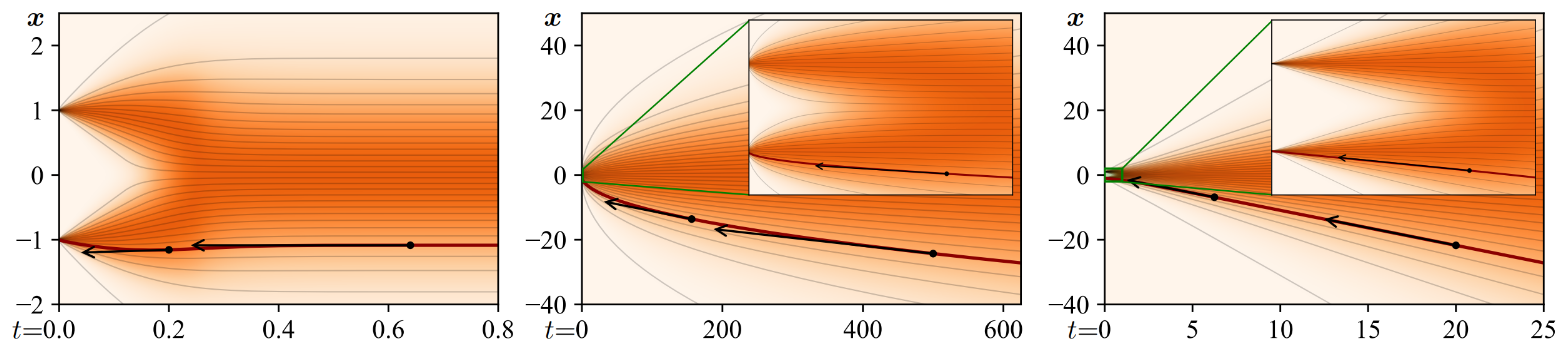
\includegraphics[width=\textwidth]{images/EDM_Sampler.png}
  }
  \caption{ A sketch of ODE curvature in 1D where \(p_{\text{data}}\) is two Dirac peaks at \(x\pm1\) Horizontal \(t\) axis is chosen to show \(\sigma\in[0,0.25]\) in each plot, with insets showing \(\sigma\in[0,1]\) near the data. Example local gradients are shown with black arrows. \emph{Left.} Variance preserving ODE of Song et al. \cite{song2021score} has
solution trajectories that flatten out to horizontal lines at large \(\sigma\). Local gradients start pointing towards data only at small \(\sigma\). \emph{Center.} Variance exploding variant has extreme curvature near data and the solution trajectories are curved everywhere. \emph{Right.} With the schedule used by DDIM \cite{song2021denoising} and us, as
\(\sigma\) increases the solution trajectories approach straight lines that point towards the mean of data. As \(\sigma \rightarrow 0\), the trajectories become linear and point towards the data manifold. Source: Karras et al.\ \cite{karras2022elucidating}.}
  \label{fig:karras_sampler_image}
\end{figure}

\textbf{Sampler design} \quad
At inference time, EDM employs a deterministic second-order Heun ODE solver with 
a $\rho$-power noise schedule:
\begin{equation}
    \label{eq:edm_sampler}
    \sigma_i = \left(\sigma_{\text{max}}^{1/\rho} + \frac{i}{N-1}
\left(\sigma_{\text{min}}^{1/\rho} - \sigma_{\text{max}}^{1/\rho}\right)
\right)^{\!\rho}, \quad i = 0, \dots, N-1
\end{equation}
with $\rho = 7$. The power-law schedule concentrates discretisation steps at
small $\sigma$, where the ODE curvature is highest and denoising errors have the
greatest impact on sample quality, which is why instead of \(\rho=3\) that equalize the truncation error at each step they chose higher values. This resulted in equivalent sample quality to DDPM with approximately $7\times$ fewer NFEs, and better convergence as shown in Fig.\ \ref{fig:karras_sampler_image}. Moreover, the sampler is independent of the training procedure, therefore a model trained with the EDM loss could be evaluated with any compatible ODE or SDE solver.

\textbf{Stochastic Heun Sampler} \label{sec:stochastic_heun} \quad Karras et al.\ also propose a stochastic variant of the Heun solver in which a controlled amount of noise is reinjected before each denoising step. Before applying the standard second-order Heun update, the current noise level $\sigma_i$ is temporarily inflated to
\begin{equation}
    \label{eq:stochastic_heun}
    \hat{\sigma}_i = \sigma_i\sqrt{1 + \gamma_i^2}, \qquad
    \gamma_i = \min\!\left(\frac{S_{\text{churn}}}{N},\;\sqrt{2}-1\right),
\end{equation}
and the sample is perturbed as $\hat{x}_i = x_i + \sqrt{\hat{\sigma}_i^2 - \sigma_i^2}\;\epsilon_i$ with $\epsilon_i \sim \mathcal{N}(0,I)$, before the Heun step proceeds from $(\hat{x}_i,\hat{\sigma}_i)$ to $\sigma_{i+1}$. The scalar $S_{\text{churn}} \geq 0$ is the sole stochasticity parameter: when $S_{\text{churn}} = 0$ every $\gamma_i = 0$ and the algorithm collapses to the deterministic ODE solver, while positive values allow the trajectory to briefly re-enter a higher-noise regime at each step, counteracting discretisation errors at the cost of additional noise injections.

\section{Conditional Score-Based Diffusion for Time Series (CSDI)}
\label{sec:csdi_literature}

Standard diffusion models, as described in the previous sections, learn to 
generate unconditionally from $p_{\text{data}}$. For time series imputation, or more generally for conditional generation, given a subset of conditioning observed values related to the target entries we can compute the conditional distribution $p(x^{\text{ta}} | x^{\text{co}})$. CSDI \cite{tashiro2021csdi} make this possible via a masking mechanism that is applied both at training and inference time. 

\textbf{Architectural lineage} \quad
To understand the architectural choices made in CSDI, it is useful to look at  
evolution of CSDI's backbone. PixelCNN \cite{oord2016pixel} established the core 
ideas of modeling high-dimensional data through local conditional information by using masked convolutions, residual connections, and gated activations, enabling the understanding of local and global relationships. WaveNet \cite{oord2016wavenet} transferred 
this logic from images to raw audio by replacing 2D masked image convolutions 
with 1D causal dilated convolutions, allowing the receptive field to grow exponentially with depth while maintaining causality. DiffWave 
\cite{kong2021diffwave} then kept the WaveNet-style residual architecture but abandoned the autoregressive component entirely, since it moves to a diffusion model. Because during denoising the target is the entire signal, future context is accessible to the model, and causal convolutions are replaced by bidirectional dilated convolutions. The key 
inherited components from WaveNet are the stacks of residual blocks, the diffusion-step conditioning, gated activations, and skip aggregation. CSDI \cite{tashiro2021csdi} then adapts this DiffWave backbone to multivariate 
time-series imputation, replacing the convolutional modeling with 
two-dimensional attention and introducing an explicit conditioning mechanism 
for observed values. The evolution therefore follows a clear progression: firstly autoregressive local dependency modelling, secondly dilated temporal convolutions, thirdly  diffusion denoising with WaveNet-style residual blocks, and then CSDI's conditional time-series denoiser with attention. 

% CSDI high-level overview
\begin{figure}[htbp]
  \centering
  {\small
  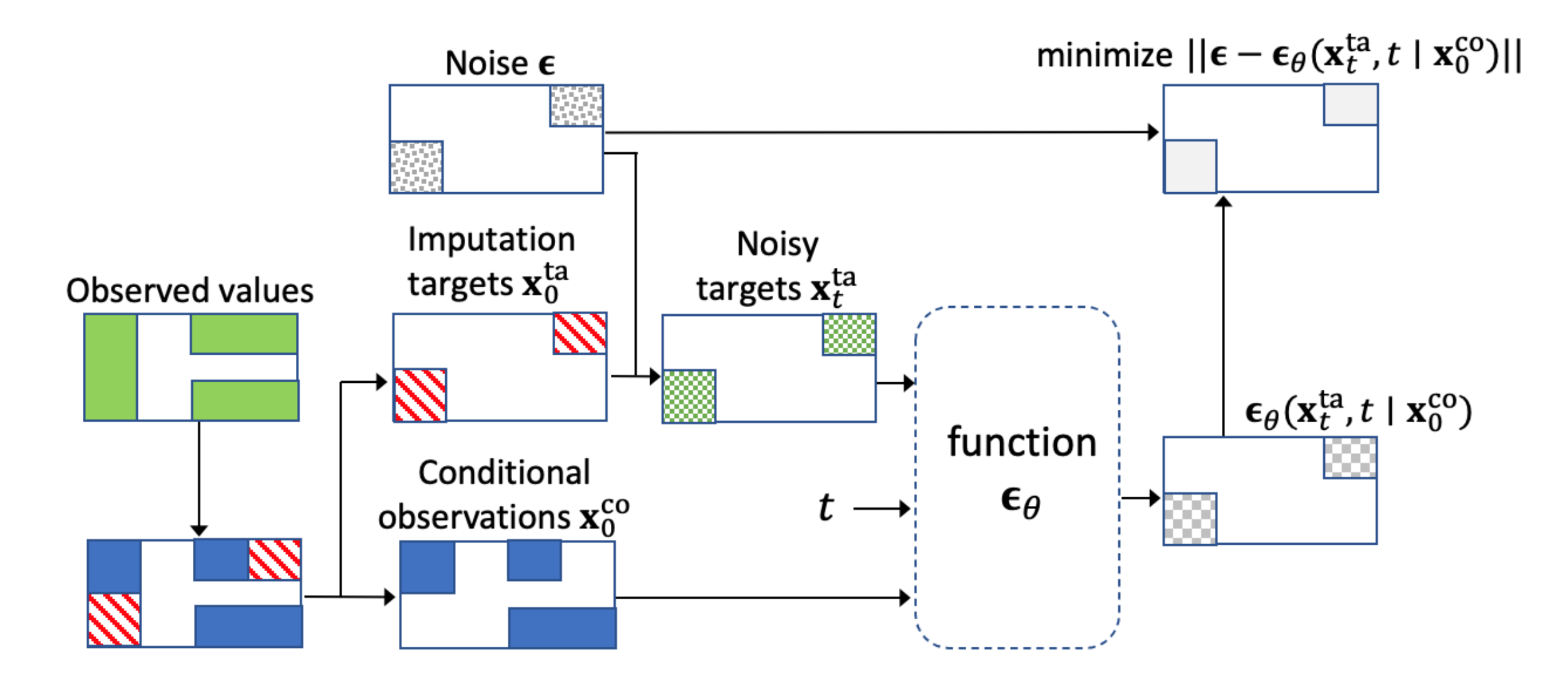
\includegraphics[width=\textwidth]{images/CSDI_high_level_overview.png}
  }
  \caption{The self-supervised training procedure of CSDI for implementation of time series imputation. The colored areas in each rectangle represent the existence of values. The green and white areas represent observed and missing values, respectively, and white areas are padded with zeros to fix the shape of the inputs. Zero padding is also applied to all white areas. As with Figure 2, the observed values are separated into red imputation targets \(x_0^{\text{ta}}\) and blue conditional observations \(x_0^{\text{co}}\). For the extended targets \(\hat{x}_0^{\text{ta}}\), the area of value 0 shows dummy values. Source: CSDI\ \cite{tashiro2021csdi}.}
  \label{fig:csdi_high_level}
\end{figure}

\textbf{Conditional denoising mechanism} \quad At each denoising step $t$, the CSDI model takes as input three quantities: 
the noisy target $x^{\text{ta}}_t$, which gets zero-padded at conditioning indices; the 
clean conditioning observations $x^{\text{co}}_0$, which gets zero-padded at target indices; and a binary mask $m^{\text{co}} \in \{0,1\}^{K \times L}$ indicating which entries are observed, where $K$ is the number of channels and $L$ is the sequence length. The conditional score network is therefore 
$\epsilon_\theta(x^{\text{ta}}_t, t \mid x^{\text{co}}_0, m^{\text{co}})$, and 
the training objective is:
\begin{equation}
\label{eq:csdi_objective}
    \min_\theta\; \mathbb{E}\left[\left\|\epsilon - 
    \epsilon_\theta\!\left(x^{\text{ta}}_t, t \;\middle|\; 
    x^{\text{co}}_0, m^{\text{co}}\right)\right\|^2_{m^{\text{ta}}}\right]
\end{equation}
where $\|\cdot\|^2_{m^{\text{ta}}}$ denotes that the squared error is evaluated 
only at target indices. The conditioning information $x^{\text{co}}_0$ and 
$m^{\text{co}}$ are kept fixed throughout the reverse process, while only the 
target entries are denoised. 

% CSDI high-level overview
\begin{figure}[htbp]
  \centering
  {\small
  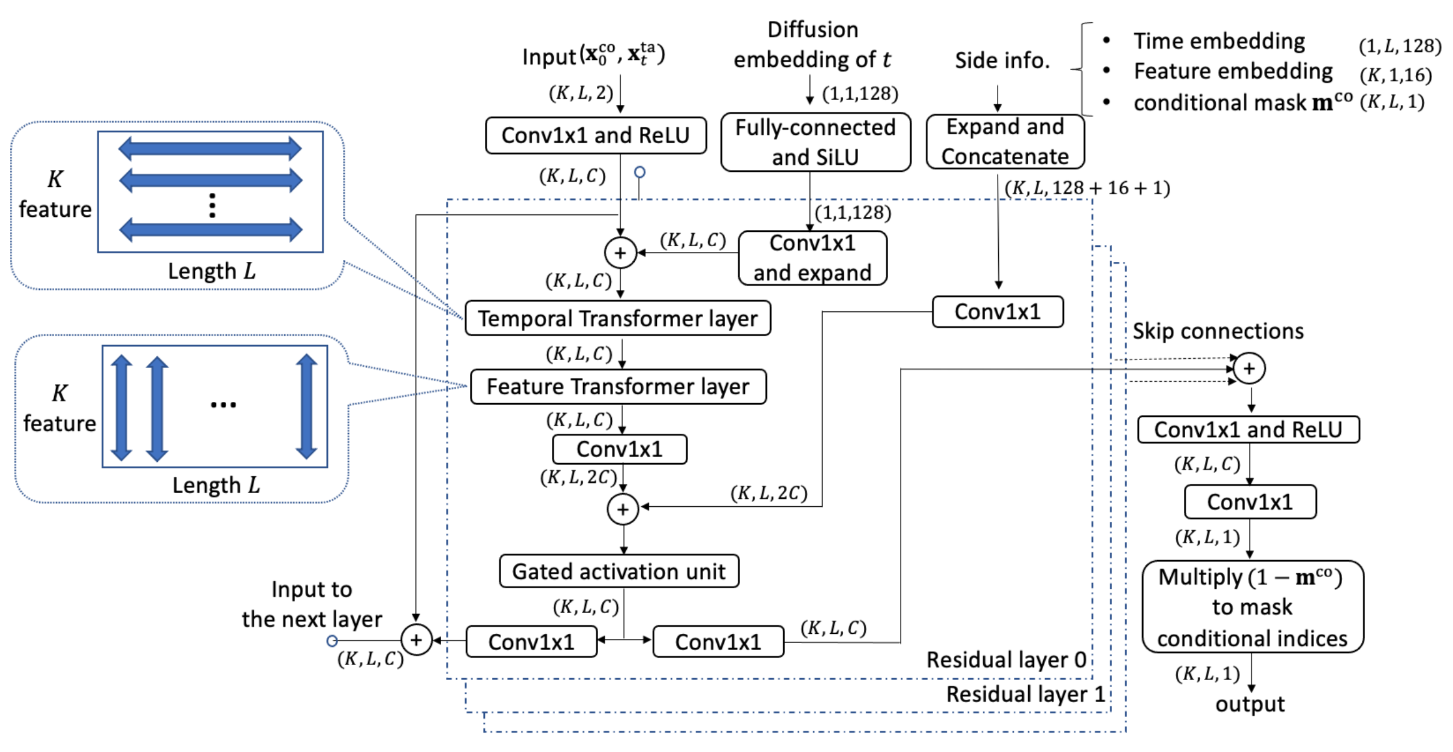
\includegraphics[width=\textwidth]{images/CSDI_architecture_full.png}
  }
  \caption{Architecture of \(\epsilon_\theta\) in CSDI for multivariate time series imputation. Source: CSDI\ \cite{tashiro2021csdi}.}
  \label{fig:csdi_high_level}
\end{figure}

\textbf{2D attention over time and features} \quad The central innovation of CSDI over DiffWave is the replacement of dilated 
temporal convolutions with a two-dimensional attention mechanism. Two Transformer 
layers \cite{vaswani2017attention} operate in sequence within each residual block: a temporal Transformer which operates along the time axis, capturing short- and long-range temporal dependencies within each channel, and a feature Transformer operating along the channel axis, capturing cross-channel dependencies between variables. This 2D attention allows the model to learn both the temporal dynamics of each channel and the 
contemporaneous relationships between channels, without the quadratic cost of 
attending jointly over the full time-feature product space. The overall block 
structure residual connections, skip aggregation, and gated activations 
is inherited directly from DiffWave and ultimately from WaveNet. 

\textbf{Positional and diffusion-step embeddings} \quad Three types of embeddings are added to the latent representation to allow the model to simultaneously distinguish temporal position, noise level, and channel 
identity: a sinusoidal diffusion-step embedding encoding the current noise level 
$t$; a temporal embedding encoding absolute position along the time axis; and a 
feature embedding encoding the identity of each channel. The diffusion-step 
embedding plays the same role as the noise conditioning $c_{\text{noise}}(\sigma)$ 
in the EDM preconditioning, ensuring that the denoiser is aware of the current noise level. 

\textbf{Self-supervised training strategy and limitations} \quad CSDI introduces several masking strategies for training (random, historical, 
mixed, and test-pattern) that simulate different conditioning and target splits 
during training, effectively providing a sort of data augmentation through varied 
masking.

\section{GBM--style SDE}
\label{sec:gbm_sde_ch2}
The idea of using CSDI for FTS modeling was explored previously by Gihum Kim et al. in \emph{A diffusion-based generative model for financial time series via geometric Brownian motion} \cite{kim2025diffusion}. While interesting this work lack the details needed in order to be replicable and provide ambiguous statements about what is actually persue. 

They showed that starting from the Black--Scholes equation (Eq.~\ref{eq:blackscholes}) and 
applying It\^{o}'s lemma to \(X_t = \log S_t\), one obtains:
\[
    dX_t = \left(\mu_t - \frac{1}{2}\nu_t^2\right)dt + \nu_t\,dW_t,
\]
where \(\nu_t > 0\) is the instantaneous volatility. Choosing 
\(\mu_t = \frac{1}{2}\nu_t^2\) cancels the drift term, yielding a 
VE-type SDE in log-price space (Eq.~\ref{eq:ve}), with the forward 
process reduced to:
\begin{equation}
    \label{eq:forward_ve}
    x_t = x_0 + \sigma\epsilon, \quad \epsilon \sim \mathcal{N}(0, I),
\end{equation}
where \(\sigma\) denotes the noise level at diffusion step \(t\), 
distinct from the instantaneous volatility. 

It is important to stress that this drift cancellation is a deliberate 
modelling choice, not a consequence of the GBM dynamics: the resulting 
process is no longer a pure GBM but rather a VE-type diffusion in 
log-price space inspired by it. The financial interpretation is that, 
while noise remains additive in log-price space, the exponential map back to price space induces effective heteroskedasticity with volatility that scales with the price level.

However, an ambiguity in the original paper requires clarification. In Section 3.1, 'Geometric Brownian motion in score-based Models' is stated:
\begin{quote}
    \emph{[...] the GBM-based formulation naturally injects larger noise into higher--value regimes, thereby preserving economically meaningful dynamics in the generated trajectories. It inherently scales noise with the underlying price level, enhancing the model’s sensitivity to large market movements. As a result, the diffusion process can more accurately capture stylized facts such as volatility clustering and heavy tails.}
\end{quote}
Nevertheless, in Section 3.1.2, the authors state:
\begin{quote}
    \emph{For each selected stock, we calculated daily log-returns, defined 
    as \(r_t = \log(p_t / p_{t-1})\), where \(p_t\) represents the 
    adjusted closing price on day \(t\). To create training samples 
    suitable for diffusion modeling, we applied a sliding window approach 
    to the log-return sequences.}
\end{quote}
This indicates that the model is trained on log-returns, not on log-prices. 
Log-prices \(X_t = \log S_t\) are non-stationary, making them undesirable 
as direct training targets. The GBM-style diffusion derivation above 
operates on log-prices in theory, but practical training on log-returns.

\section{Heavy--Tailed Diffusion Models}

A natural question follows from the heavy--tailed nature of financial time series: if the target distribution exhibits rare but economically important extreme events, should the forward perturbation process also be heavy--tailed, so that both the noised data and the terminal prior better reflect the structure of the underlying data structure.

This question remains open in literature, but in order to narrow down the problem we should consider the following points:
\begin{itemize}
    \item Can a diffusion model based on Gaussian perturbations learn a heavy--tailed target distribution at all?
    \item If it can, how much modelling capacity should be explicitly allocated to tail behaviour rather than to the bulk of the distribution?
\end{itemize}
Recent theoretical work suggests that Gaussian perturbations are not automatically invalid in the presence of heavy tails. Yu et al.\ \cite{yu2026diffusion} study standard Gaussian score-based diffusion models when the target distribution is heavy--tailed. Under a tractable kernel-based score estimator, they derive minimax guarantees showing a distinction between tail regimes: for exponentially decaying tails, Gaussian diffusion remains statistically robust, while for polynomially decaying tails the score-estimation and sampling rates depend explicitly on the tail index. Since financial log-returns are commonly modelled as having polynomial-like tail decay, this result is directly relevant to financial time series. It does not imply that Gaussian diffusion is unusable, but it does indicate that heavy tails increase the statistical difficulty of score learning. 

A complementary line of work modifies the perturbation distribution itself. Pandey et al.\ \cite{pandey2024heavytailed} propose heavy--tailed diffusion models based on multivariate Student-\(t\) perturbation kernels, leading to \(t\)-EDM. In this framework, the degrees-of-freedom parameter \(\nu\) controls tail heaviness: smaller values of \(\nu\) produce heavier tails, while the Gaussian case is recovered in the limit \(\nu \to \infty\). Because the Kullback--Leibler divergence between Student-\(t\) distributions does not generally admit a convenient closed form, they replace the usual KL-based objective with a \(\gamma\)-power divergence. This objective is not an ELBO in the standard sense, but it recovers the KL divergence in the appropriate limited regime. 

A more radical alternative is to replace Brownian motion itself with a heavy--tailed jump process. Yoon et al.\ \cite{yoon2023score} propose the L\'evy-It\^o Model, which uses isotropic \(\alpha\)-stable L\'evy processes instead of Brownian motion. They derive the corresponding reverse-time SDE and train the model through fractional denoising score matching. Such an approach is conceptually appealing for financial data, where jumps and rare events are structurally important. However, it requires a different and specific score object and reverse process, as well as a substantially different mathematical framework from the Gaussian EDM--CSDI model used in this work. This does not gurantee the same freedom for design choices as EDM.

Consequently, this thesis study a Gaussian EDM--CSDI baseline for conditional financial time-series generation, with explicit tail-sensitive evaluation. Heavy--tailed perturbation kernels and L\'evy-driven score models may improve tail fidelity, but they also introduce additional modelling choices and may alter the trade-off between tail accuracy, bulk distributional fit, training stability, and computational simplicity.
% \section{Summary}

% This chapter has established the theoretical foundations upon which the present work is built. We began by characterising financial time series through their core stylized facts and discussed the related challenges with modeling such properties. Subsequently, we presented the classical approaches GARCH and Merton's jump diffusion, along with their ability to capture some of these features through parametric assumptions, and their structural limitations. 

% Deep generative models lift this restriction, but GANs and VAEs introduce their own pathologies, in particular mode collapse and over-smoothing, respectively, that are particularly damaging in the heavy-tailed, asymmetric setting such as financial returns. Score-based diffusion models offer a more principled alternative: a stable training objective grounded in denoising score matching, a well-understood probabilistic framework, and the flexibility to condition generation on partial observations. 

% Within this family, the EDM framework of Karras et al.\cite{karras2022elucidating} provides a structured decomposition of the design space by using preconditioning, loss weighting, noise distribution, and sampler, that resolves several heuristic choices left open by DDPM and Song et al. \cite{ho2020ddpm, song2021score}. CSDI \cite{tashiro2021csdi} then introduces the conditional masking mechanism and the factored two-dimensional attention architecture that make conditional generation over multivariate time series more feasible. Together, these two frameworks form the direct theoretical basis of this thesis, which combines EDM preconditioning and loss weighting with a CSDI-style backbone to generate conditional values. 

% A prior attempt to unify these ideas in a financial setting was made by Kim et al.\cite{kim2025diffusion}, who derived a VE-type forward process from GBM dynamics by cancelling the drift term in log-price space and applying CSDI as the backbone. While conceptually motivated, the paper contains reproducibility limitations and a notable internal inconsistency: the theoretical derivation operates on log-prices, yet the reported experiments train on log-returns. Furthermore, claims that the GBM formulation inherently captures volatility clustering and heavy tails are overstated: once the model is trained on log-returns rather than log-prices, the price-level scaling that motivates those claims no longer applies directly to the training signal. The present work takes this prior contribution as context and background, adopts the same CSDI backbone, but replaces the VE-style SDE formulation with the EDM framework, which offers a more principled and flexible treatment of the noise schedule, preconditioning, and loss weighting.

\chapter{Theoretical Framework}
\label{ch:theoretical_framework}
The following chapter builds on the previous one, detailing the theoretical structure and motivation for the implemented model.

\section{Adapting the Framework to OHLC Financial Time Series}
\label{sec:ohlc_theoretical}

\(\textbf{Phase 1}\quad\) Data are formally represented as \(X \in \mathbb{R}^{K \times L}\), where \(K\) denotes the number of channels and \(L\) the number of time steps per window. In Phase~1, \(K = 1\) and the input reduces to a univariate sequence of Close log-returns.

\(\textbf{Phase 2}\quad\) OHLC have \(K = 4\) which denotes the number of channels (Open, High, Low, Close), or conditioning features. This partition is 
financially motivated: the opening price \(O_t\) is fixed at the start of 
the trading session, while the intraday extremes \(H_t\) and \(L_t\) are 
continuously observed throughout it, encoding both the direction of price 
movements and the microstructure of intraday volatility. The closing price 
\(C_t\), by contrast, is determined only at the end of the session. Two 
derived quantities are particularly informative as conditioning signals: the 
overnight return \(O_t / C_{t-1}\), which captures the opening gap with 
respect to the previous close, and the intraday range \(H_t - L_t\), a 
well-established realised volatility proxy \cite{parkinson1980extreme}. In addition, log-returns are often preferred to nominal prices because of their stationarity \cite{cont2001empirical}, which makes them comparable across time and assets, removing underlying price trends.

According to what stated before data can be partitioned into a conditioning set 
\(\mathcal{C} = \{O, H, L\}\) and a target set \(\mathcal{T} = \{C\}\), 
and the model is trained to learn the conditional distribution
\[
    p\!\left(X^{\text{ta}} \mid X^{\text{co}} = x^{\text{co}}\right),
\]
where \(X^{\text{ta}}\) denotes the Close channel and \(X^{\text{co}}\) 
denotes the observed OHL channels. 

Daily prices are constrained by the ordering relationship 
\(L_t \leq \min(O_t, C_t) \leq \max(O_t, C_t) \leq H_t\). 
When the series is expressed as log-returns (Eq.\ref{eq:log_returns}), this constraint no longer 
admits a closed form, since it involves nonlinear inequalities across cumulative sums of returns rather than individual observations. 
Nevertheless, it remains a building structural property of the 
data-generating process. On the other hand, because the Gaussian diffusion kernel has 
unbounded support, there is no guarantee that generated Close values 
will respect the implied bounds \([L_t,\, H_t]\). No constraint-preserving 
mechanism is applied in this work; the ordering relationship is further 
disrupted by feature-wise global normalisation, which rescales each channel independently and therefore does not preserve the relative ordering between  channels.

\section{Classical Baselines with OHLC Conditioning}
\label{sec:classical_baselines_theoretical}

As introduced in Sec.~\ref{sec:classical_models_literature}, GARCH and Merton
models serve as parametric benchmarks. Both are extended with exogenous OHLC
conditioning, denoted by the suffix \emph{-X}, so that they receive the same
per-day information as the diffusion model's conditioning set
$\mathcal{C}=\{O,H,L\}$. Each model is fitted per ticker by maximum likelihood
via L-BFGS-B.

\textbf{Log-GARCH-X with Student-$t$ Innovations} \quad The close log-return follows an AR(1) mean with log-GARCH variance: \(r_t = \mu + \phi\, r_{t-1} + \varepsilon_t\) with \(\varepsilon_t = \sigma_t z_t\) and \(z_t \sim t_\nu\), therefore we are modeling:
\[
\log \sigma_t^2 = \omega + \alpha \log(\varepsilon_{t-1}^2 + c)
        + \beta \log \sigma_{t-1}^2 + \boldsymbol{\delta}^\top \mathbf{q}_t
\]
with $|\phi|<0.5$, $\alpha+\beta<0.98$, and $\nu>2$. The log-GARCH
formulation keeps $\sigma_t^2$ positive by construction without any sign
constraints on $(\omega,\alpha,\beta)$. The Student-$t$ innovations is used to better capture fat tails. The OHLC conditioning vector is:
\[
    \mathbf{q}_t = \Bigl[ o_t^2,\;
    \tfrac{(\log H_t/L_t)^2}{4 \log 2} \Bigr]^\top,
\]
where $o_t^2$ is the squared overnight log-return and the second term is
the Parkinson~\cite{parkinson1980extreme} realised variance estimator
(App.~\ref{app:baselines} for more details).

\textbf{Merton-X} \quad The close log-return is decomposed into a diffusive and a compound Poisson
component:
\[
    \label{eq:mertonx_return}
    r_t = \mu + \nu_t Z_t + \sum_{i=1}^{P_t} Y_{t,i}, \quad
    P_t \sim \operatorname{Poisson}(\lambda), \quad
    Y_{t,i} \sim \mathcal{N}(\mu_J, \sigma_J^2),
\]
where the diffusive volatility $\nu_t$ is driven by observations:
\begin{equation}
    \label{eq:mertonx_logvar}
    \log \nu_t^2 = a_0 + \mathbf{a}^\top \mathbf{q}_t, \qquad
    \mathbf{q}_t = \bigl[o_t^2,\; (\log H_t/L_t)^2\bigr]^\top.
\end{equation}
Unlike GARCH-X, there is no sequential recursion: $\nu_t$ depends only on
same-day observables, making the inference structure directly analogous to the
diffusion model's use of $\{O_t, H_t, L_t\}$ to generate $C_t$.
It is well established that marginalising over Poisson counts results in a Gaussian mixture likelihood (App.~\ref{app:baselines}). 

Both baselines are parametric and trained globally per each ticker's full
history, therefore they are ticker specific. Moreover, capture complementary stylized facts — volatility clustering and
heavy tails in GARCH-X, sudden discontinuities in Merton-X — but neither
learns the conditional distribution $p(r_t^C \mid r_t^O, r_t^H, r_t^L)$
non-parametrically. The diffusion model is the non-parametric alternative,
at the cost of higher complexity.

\section{SDE and the VE Instantiation}
As discussed in Sec.~\ref{sec:scorediffmodels}, diffusion models were 
originally developed in distinct formulations before being unified under 
the EDM framework. These structures are relevant for Phase~1, which aims to replicate the results of Kim et al.\cite{kim2025diffusion}. Meanwhile, for Phase~2 we will move towards the EDM framework.

\(\textbf{Phase 1}\quad\) Phase~1 is identical in its implementation to Song et al. in \cite{song2021score}, but in a simplified version [CITE REPOSITORY].

\(\textbf{Phase 2}\quad\) For Phase~2, we can look at the forward VE formulation, Eq.\ref{eq:reverse_sde}, the corresponding reverse SDE for VE case is \[dx=-\sigma\nabla_x \log p_\sigma(x)\] when defined in \(\sigma\)-space (with \(\sigma\) decreasing) instead of \(t\)-space, due to EDM conditioning modeling choices. With the deterministic counterparts, the probability flow ODE is:
\[
\frac{dx}{d\sigma}=-\frac{\sigma}{2}\nabla_x\log p_\sigma(x)
\]

As discussed in Sec.\ref{sec:scorediffmodels} we can use DSM to brigde the gap between denoising and score matching. It turned out that DSM is a special case of a statistical result known as Tweedie’s formula, which provides a relationship between score functions and conditional expectations. For noisy observation Eq.\ref{eq:forward_ve} the optimal MMSE denoiser is:
\[
D^*(x_t;\sigma)=\mathbb{E}\left[X_0|X_t=x_t\right]
\]
therefore denoiser and score function are connected by:
\[
\nabla_{x_t}\log p_\sigma(x_t)=\frac{D^*(x_t;\sigma)-x_t}{\sigma^2}
\]
implying that rather than learn the score field directly, which is hard and ill-conditioned regression target in high dimensions, we train a denoiser \(D_\theta\) to approximate \(D^*\), and we later recover the score analytically.

\section{GBM--style SDE and CSDI}
\label{sec:gbm_sde_ch3}
In Sec.\ref{sec:gbm_sde_ch2} we mentioned the 
cumulative interpretation of log-returns, which stands from the fact that training diffusion models on raw log-prices $X_t = \log S_t$ is inadvisable 
for two reasons. First, log-prices are non-stationary, therefore their mean grows approximately linearly and with different scales across tickers and time periods. Second, the sampling process relies on a Gaussian prior 
$\mathcal{N}(0, \sigma_{\max}^2 I)$ that should be well-matched to the training distribution, which in this case means only if the data input is approximately centered at zero with a scale commensurate with $\sigma_{\max}$. 
Raw log-prices violate both conditions significantly. Daily log-returns 
$r_t = \log(S_t / S_{t-1})$ solve non-stationarity, however, 
working with cumulative log-returns 
$\mathcal{C}_{\tau+k} = \sum_{j=1}^{\tau+k} r_j$ 
is motivated by the GBM theoretical derivation of Sec.~\ref{sec:gbm_sde_ch2} and by the experimental results shown in Figures~4--6 of \cite{kim2025diffusion}, that otherwise wouldn't have any reason to differentiate VE with GBM. How non--stationarity of cumulative log-returns is handled is addressed in Sec.\ref{sec:sliding_window_ch4}.

\begin{figure}[htbp]          % placement: here, top, bottom, page
  \centering
  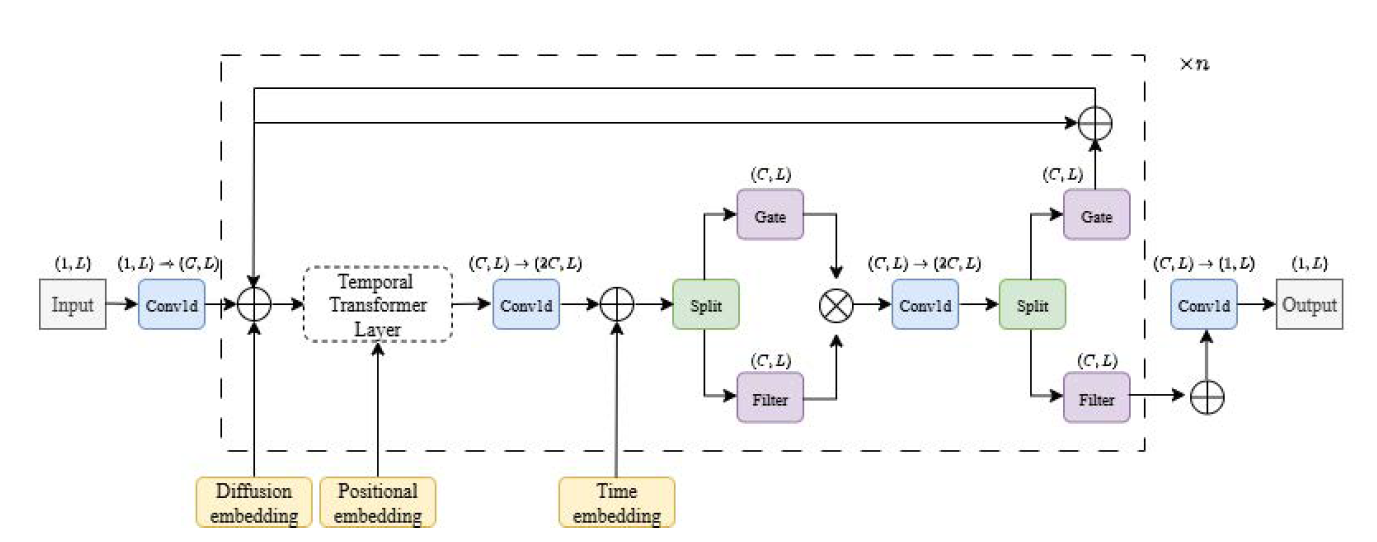
\includegraphics[width=0.9\textwidth]{images/Kim_et_al_architecture.png}
  \caption{CSDI-based diffusion architecture. Source: Kim et al.\ \cite{kim2025diffusion}.}
  \label{fig:kim_architecture}
\end{figure}

Another inconsistency arises between the described use of time, positional, and diffusion-step embeddings. The text states that
\begin{quote}
    \emph{These embeddings are added to the latent representation and passed through a Transformer block, which models global dependencies across time.}
\end{quote}
However, Fig.\ref{fig:kim_architecture} clearly shows that the time embeddings is provided only after the Transformer layer. This last interpretation was used. 

Based on the model architecture presented in Fig.\ref{fig:kim_architecture}, the diffusion-step, temporal, and positional embeddings were interpreted as being injected independently at every residual block, consistently with the approach adopted in CSDI \cite{tashiro2021csdi}. This reading is further supported by Fig.\ref{fig:kim_architecture} itself, their position is probably justified by the fact that they are computed once. Notably, Kim et al.\ \cite{kim2025diffusion} describe the time embedding as combining sinusoidal functions with learnable vectors, while the positional embedding relies solely on fixed sinusoidal functions with no learnable parameters; this distinction suggests that the positional embedding is the only one among the three that contains no trainable weights. 

% The authors Kim et al.\cite{kim2025diffusion} did not release a common dataset, source code, or key implementation details, including data pre-processing, the masking strategy, the model’s loss function or prediction target, kernel size, transformer hyperparameters, optimizer configuration, and others. All these aspects will be examined in detail in Ch.\ref{ch:data_setup}.

\section{EDM}
The components described in this section apply exclusively to Phase~2.

\textbf{Preconditioning} Training a raw network \(F_\theta (x_t;\sigma)\) directly as a denoiser is impractical because according to 
Eq.\ref{eq:forward_ve} the inputs have variance \(\sigma_{\text{data}}+\sigma^2\), which means that the network sees input that varies by orders of magnitude across the distribution of \(\sigma\), which display different noise levels, as discussed in Sec.\ref{sec:edm_literature}. EDM addresses both problems introducing preconditioned denoiser \(D_\theta\) (Eq.\ref{eq:edm_denoiser}). 

Follows the role of each preconditioning parameter:
\begin{itemize}
    \item \(c_{\text{in}}(\sigma)\), input normalization: \(F_\theta\) receives as input \(c_{\text{in}}(\sigma)\cdot x_t\), and because, according to Eq.\ref{eq:forward_ve}, \(\operatorname{Var}(x_t)=\sigma_{\text{data}^2}+\sigma^2\), then we scale the input to unit variance.
    \item \(c_{\text{skip}}(\sigma)\), skip connection: is the Wiener filter coefficient, or the optimal linear estimator of \(x_0\) given \(x_t\). This is dervied from the MMSE argument, and it controls how much of the noisy input is passed directly to the output.
    \item \(c_{\text{out}}(\sigma)\), output scaling: rescales the network output so that the effective training targets also have unit variance, similarly to \(c_{\text{in}}(\sigma)\).
\end{itemize}

\begin{figure}[htbp]          % placement: here, top, bottom, page
  \centering
  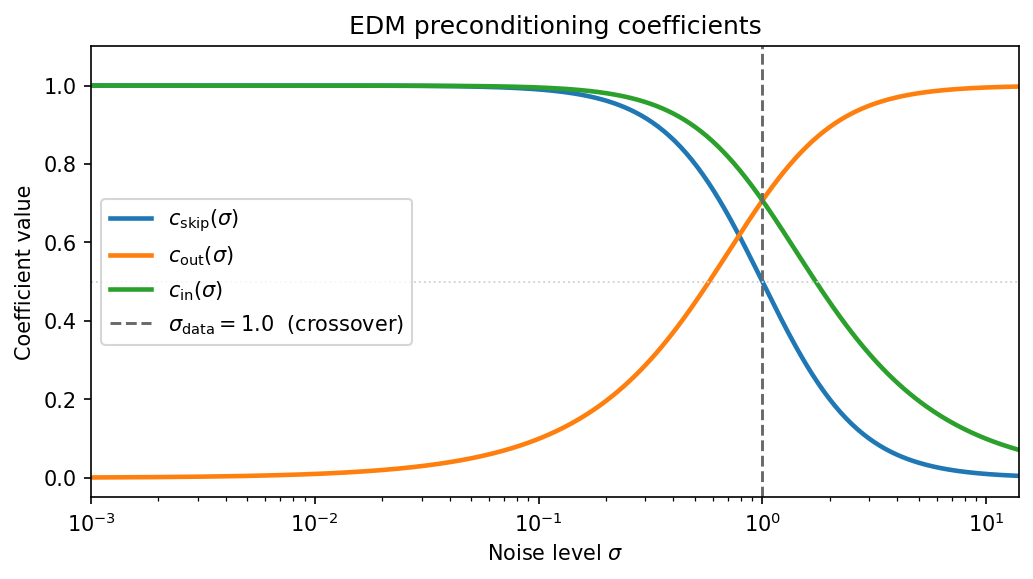
\includegraphics[width=0.6\textwidth]{images/preconditioning.png}
  \caption{Preconditioning coefficients for \(\sigma_{\text{data}}=1\), with \(\sigma_{\min}=0.002\) and \(\sigma_{\max}=7.0\).}
  \label{fig:preconditioning}
\end{figure}
In summary, \(c_{\text{skip}}(\sigma)\cdot x\) is the linear prior, while \(c_{\text{out}}(\sigma)\cdot F_\theta(\cdot)\) is the non-linear correction on top of the prior. It is important to pay attention at the crossover point where \(\sigma=\sigma_{\text{data}}\) and \(c_{\text{skip}}(\sigma)=0.5\), meaning both terms contributes equally. For instance, with \(\sigma_{\text{data}}=1\) then if \(\sigma<1\), the network makes tiny corrections and if \(\sigma>5\), the network reconstruct almost entirely from noise. 

% [IMAGE OF THE CURVES FOR sigma\_data=1 AND OTHER SIGMAS] 

\(c_{\text{noise}}(\sigma)\) is not derived from a requirement, but it is empirically chosen for numerical stability, and it is used to compresses the large dynamic range of \(\sigma\) into a bounded scalar, where the \(\frac14\) prevents saturation of the network's embedding layer. This actually is connected to CSDI's diffusion--step embedding (Sec.\ref{sec:model_architecture}), since it encodes the noise level for the network. 


\textbf{Sigma distribution} The EDM framework was originally calibrated on ImageNet \cite{deng2009imagenet} 
with \(\sigma_{\text{data}} = 0.5\), \(P_{\text{mean}} = -1.2\), and 
\(P_{\text{std}} = 1.2\). These defaults reflect the pixel-value statistics 
of natural images after unit-variance normalisation. OHLC log-returns differ 
in a relevant respect: after global standardisation, each channel has unit 
variance by construction, so \(\sigma_{\text{data}} = 1.0\) is the 
appropriate choice. It is important to notice that \(P_{\text{mean}}\) shift the distribution, where lower values concentrate training on fine-grained reconstruction, and viceversa. \(P_{\text{std}}\) control the spread, where wider spread gives more uniform coverage. It is important that the \(\sigma_{\max}\) used for the prior sampling in the reverse process, covers approximately 95\% or more of the distribution \(\ln (\sigma)\sim \mathcal{N}(P_{\text{mean}}, P_{\text{std}})\). Whether \(P_{\text{mean}}\) and \(P_{\text{std}}\) 
also have empirically optimal values for this domain remains an open calibration question only partially addressed in this work. 

\textbf{Loss function} EDM varies also the loss function characterization by moving away from noise prediction as in Eq.\ref{eq:csdi_objective}, to a "clean" data prediction, Eq.\ref{eq:edm_loss}, with different weighting, as discussed in Sec.\ref{sec:edm_literature}.

\section{Architecture}
\label{sec:model_architecture}
The CSDI-based backbone described in this section is shared by both phases.

U-Net architectures \cite{ronneberger2015unet} have been widely adopted 
in diffusion models for image generation, where hierarchical downsampling 
and convolutional inductive biases provide strong local structure and 
multi-scale spatial representations. Financial time series, however, are 
not characterised by local spatial regularity but by long-range temporal 
dependencies and contemporaneous cross-channel relationships, for which 
the locality assumptions of convolutions are a poor fit. Transformers, by 
contrast, attend globally over the input, making them 
theoretically better suited to this domain. 

As discussed in Sec.~\ref{sec:csdi_literature}, CSDI factors the full 
\(K \times L\) attention into a temporal Transformer operating over 
\(L \times L\) and a feature Transformer operating over \(K \times K\), 
reducing complexity from \(\mathcal{O}\!\left((KL)^2\right)\) to 
\(\mathcal{O}(L^2 + K^2)\). Beyond computational savings, the factored design is also 
structurally motivated: temporal attention captures \emph{when} patterns 
occur within each channel, while feature attention captures \emph{how} 
channels covary contemporaneously. Attending jointly over the time-feature 
product space would mix these two distinct dependency 
types, making the learned representations harder to interpret and 
potentially trickier to optimise. 

A general functioning approach is illustrated in Fig.\ \ref{fig:csdi_overview}. Were inputs, specifically \(\sigma\), noised data \(x_t\), observed_data or data that does not need inputation,
cond_mask which defines which data are conditional, and observed_tp or indices (time) available are passed to the denoiser at different stages, as described in Fig.\ \ref{fig:model_input}. Then inputs pass through a series of \(n\) \texttt{ResidualBlock} and finally the Denoiser output \(F_\theta(c_{\text{in}}(\sigma)x; c_{\text{noise}(\sigma)}), \).
It follows a more detailed explanations about the components, specifically those that constitute the \texttt{ResidualBlock} represented in Fig.\ \ref{fig:csdi_residual_block}.

% % THE GRAPHS ARCHITECTURES ARE HERE

%DO NOT PRINT \begin{figure}[h]
    \centering
    \begin{tikzpicture}[
        font=\small,
        >=Latex,
        node distance=0.65cm and 2.0cm,
        mainblock/.style={
            draw=blue!70!black,
            fill=blue!12,
            rounded corners=3pt,
            minimum width=3.8cm,
            minimum height=0.8cm,
            align=center,
            thick
        },
        ioblock/.style={
            draw=black,
            fill=red!10,
            rounded corners=2pt,
            minimum width=3.8cm,
            minimum height=0.75cm,
            align=center
        },
        sideblock/.style={
            draw=black!60,
            fill=gray!12,
            rounded corners=2pt,
            minimum width=2.8cm,
            minimum height=0.7cm,
            align=center
        },
        resbox/.style={
            draw=black!75,
            fill=gray!7,
            rounded corners=5pt,
            minimum width=3.8cm,
            minimum height=2.2cm,
            align=center,
            thick
        },
        skipblock/.style={
            draw=black!60,
            fill=yellow!18,
            rounded corners=2pt,
            minimum width=3.0cm,
            minimum height=0.72cm,
            align=center
        },
        arr/.style={->, thick},
        sarr/.style={->, thick, dashed}
    ]

    \node[ioblock] (xin) {
        $\mathbf{x}_t,\;\mathbf{m}$\\
        \scriptsize$(B,\,2,\,K,\,L)$
    };

    \node[mainblock, below=of xin] (inproj) {
        \textbf{input\_projection}\\
        \scriptsize Conv1d $2\!\to\! d$,\;$k{=}1$
    };

    \node[resbox, below=of inproj] (resblocks) {
        \textbf{ResidualBlock}\\
        $\times\,n_{\mathrm{layers}}$\\[2pt]
        \scriptsize(see Fig.~\ref{fig:csdi_residual_block})
    };

    \node[skipblock, below=of resblocks] (skippool) {
        $\displaystyle\sum_{\ell}\,\mathrm{skip}_{\ell}\,/\,\sqrt{n}$
    };

    \node[mainblock, below=of skippool] (outproj) {
        \textbf{output\_projection}\\
        \scriptsize Conv1d $d\!\to\!1$,\;$k{=}1$
    };

    \node[ioblock, below=of outproj] (xout) {
        $\hat{\mathbf{x}}_0$\\
        \scriptsize$(B,\,1,\,K,\,L)$
    };

    \node[sideblock, left=of resblocks] (cnoise) {
        $c_{\mathrm{noise}}(\sigma)$\\
        \scriptsize diffusion emb.
    };

    \node[sideblock, right=of resblocks] (sideinfo) {
        \textbf{side\_info}\\
        \scriptsize time + feature emb.
    };

    \draw[arr] (xin)       -- (inproj);
    \draw[arr] (inproj)    -- node[right, font=\scriptsize] {$(B,d,K,L)$} (resblocks);
    \draw[arr] (resblocks) -- node[right, font=\scriptsize] {accumulated skips} (skippool);
    \draw[arr] (skippool)  -- (outproj);
    \draw[arr] (outproj)   -- (xout);

    \draw[sarr] (cnoise.east)   -- (resblocks.west);
    \draw[sarr] (sideinfo.west) -- (resblocks.east);

    \end{tikzpicture}
    \caption{High-level overview of the CSDI denoising network. The noisy observation $\mathbf{x}_t$ and its binary mask $\mathbf{m}$ are lifted into a $d$-dimensional latent space by a pointwise convolution and processed by $n_{\mathrm{layers}}$ stacked residual blocks, each conditioned on the diffusion-step embedding $c_{\mathrm{noise}}(\sigma)$ and the side information (time and feature embeddings). Skip connections from every block are accumulated and normalised before a final pointwise convolution recovers the predicted clean signal $\hat{\mathbf{x}}_0$.}
    \label{fig:csdi_overview}
\end{figure}


\begin{figure}[h]
    \centering
\begin{adjustbox}{max width=\textwidth, max height=0.92\textheight, keepaspectratio}
\begin{tikzpicture}[
    font=\small,
    >=Latex,
    node distance=0.7cm and 1.0cm,
    inputblock/.style={
        draw=black,
        fill=red!12,
        rounded corners=2pt,
        minimum width=2.8cm,
        minimum height=0.9cm,
        align=center
    },
    convblock/.style={
        draw=blue!70!black,
        fill=blue!15,
        rounded corners=2pt,
        minimum width=4.0cm,
        minimum height=1.0cm,
        align=center,
        thick
    },
    resblock/.style={
        draw=black!70,
        fill=gray!15,
        rounded corners=3pt,
        minimum width=4.3cm,
        minimum height=1.3cm,
        align=center,
        thick
    },
    opblock/.style={
        draw=black!70,
        fill=yellow!20,
        rounded corners=2pt,
        minimum width=3.5cm,
        minimum height=0.8cm,
        align=center
    },
    skipblock/.style={
        draw=black!70,
        fill=green!12,
        rounded corners=2pt,
        minimum width=3.5cm,
        minimum height=0.8cm,
        align=center
    },
    shapetext/.style={
        font=\scriptsize,
        align=center
    },
    mainarrow/.style={->, thick},
    skiparrow/.style={->, thick, dashed},
    projblock/.style={
        draw=purple!70!black,
        fill=purple!12,
        rounded corners=2pt,
        minimum width=3.7cm,
        minimum height=0.8cm,
        align=center
    },
    sidearrow/.style={->, thick, dashed}
]
% ============================================================
% MAIN ROW -- left-to-right data flow
% ============================================================
\node[inputblock] (input) {
    \textbf{Input}
};
% Moved slightly left by reducing distance from Input
\node[convblock, right=0.55cm of input] (inputproj) {
    \textbf{input\_projection}\\
    Conv1d, kernel size $1$
};
% Increased distance from input_projection so ResidualBlock remains visually separated
\node[resblock, right=2.75cm of inputproj] (residual) {
    \textbf{ResidualBlock}\\
    with skip taps
};
% Moved skip aggregation slightly to the right
\node[skipblock, right=1.75cm of residual] (sumskip) {
    $\displaystyle \sum \mathrm{skips}/\sqrt{n}$
};
\node[convblock, right=0.9cm of sumskip] (outputproj) {
    \textbf{output\_projection}\\
    Conv1d, kernel size $1$
};
\node[opblock, right=0.9cm of outputproj] (reshape) {
    $D_x = c_{\mathrm{skip}}\,x_t \;+\; c_{\mathrm{out}}\,F_x$
};
\node[inputblock, right=0.9cm of reshape] (output) {
    \textbf{Output}
};
% ============================================================
% DIMENSION LABELS -- upper-right corner of every block
% (input label removed per request)
% ============================================================
\node[shapetext, anchor=south west]
    at ($(inputproj.north east)+(-1.0,0.01)$)
    {$(B,\mathrm{ch},K,L)$};
\node[shapetext, anchor=south west]
    at ($(residual.north east)+(-1.0,0.01)$)
    {$(B,\mathrm{ch},K{\times}L)$};
\node[shapetext, anchor=south west]
    at ($(sumskip.north east)+(-1.0,0.01)$)
    {$(B,\mathrm{ch},K{\times}L)$};
\node[shapetext, anchor=south west]
    at ($(outputproj.north east)+(-1.5,0.01)$)
    {$(B,1,K{\times}L)$};
\node[shapetext, anchor=south west]
    at ($(reshape.north east)+(-1.0,0.01)$)
    {$(B,K,L)$};
\node[shapetext, anchor=south west]
    at ($(output.north east)+(-1.0,0.01)$)
    {$(B,K,L)$};
% ============================================================
% MAIN FLOW ARROWS -- left to right
% ============================================================
\draw[mainarrow] (input)      -- (inputproj);
\draw[mainarrow] (inputproj)  -- (residual);
\draw[mainarrow] (residual)   -- (sumskip);
\draw[mainarrow] (sumskip)    -- (outputproj);
\draw[mainarrow] (outputproj) -- (reshape);
\draw[mainarrow] (reshape)    -- (output);
% ============================================================
% EXTRA ARROWS FROM INPUT
% Arrow from top-center of input to top-center of ResidualBlock
% ============================================================
\draw[mainarrow]
    (input.north)
    -- ++(0, 1.4cm)
    -| (residual.north);
% Arrow from bottom-center of input to bottom-center of Reshape
\draw[mainarrow]
    (input.south)
    -- ++(0, -1.4cm)
    -| (reshape.south);
% ============================================================
% REPEATED-BLOCK ANNOTATION
% ============================================================
\node[anchor=west, font=\large]
    at ($(residual.east)+(10.0cm,1.5cm)$)
    {$\times n$};
% ============================================================
% DASHED CONTAINER -- enlarged to include input_projection,
% ResidualBlock, sumskip (skips), and output_projection.
% ============================================================
\node[
    draw=black,
    dashed,
    rounded corners=3.8pt,
    inner sep=0.55cm,
    fit=(inputproj)(residual)(sumskip)(outputproj)
] (rescontainer) {};
\end{tikzpicture}
\end{adjustbox} % end adjustbox
    \caption{High-level overview of the CSDI denoising network. The two-channel input (details in Fig.\ \ref{fig:model_input}) is projected into a latent space, processed by $n$ stacked residual blocks with skip connections, and decoded back to the predicted clean signal.}
    \label{fig:csdi_overview}
\end{figure}

% DO NOT PRINT \begin{figure}[h]
    \centering
\begin{adjustbox}{max width=\textwidth, max height=0.92\textheight, keepaspectratio}
\begin{tikzpicture}[
    font=\small,
    >=Latex,
    % ---- block styles ----
    inputblock/.style={
        draw=black, fill=red!12, rounded corners=3pt,
        minimum width=2.8cm, minimum height=0.85cm, align=center},
    edmblock/.style={
        draw=orange!80!black, fill=orange!15, rounded corners=3pt,
        minimum width=3.6cm, minimum height=1.05cm, align=center, thick},
    embedblock/.style={
        draw=teal!60!black, fill=teal!12, rounded corners=3pt,
        minimum width=3.8cm, minimum height=1.05cm, align=center, thick},
    procblock/.style={
        draw=blue!70!black, fill=blue!12, rounded corners=3pt,
        minimum width=3.6cm, minimum height=1.05cm, align=center, thick},
    convblock/.style={
        draw=blue!70!black, fill=blue!15, rounded corners=3pt,
        minimum width=3.8cm, minimum height=1.05cm, align=center, thick},
    resblock/.style={
        draw=black!70, fill=gray!15, rounded corners=4pt,
        minimum width=4.5cm, minimum height=2.5cm, align=center, thick},
    opcircle/.style={
        draw=black!75, circle, fill=white, inner sep=1pt,
        minimum size=0.65cm, font=\small, thick},
    shapetext/.style={font=\scriptsize, align=center},
    mainarrow/.style={->, thick},
    % half-block: invisible node used only for anchor geometry
    halfnode/.style={
        draw=none, fill=none,
        minimum width=2.2cm, minimum height=0.95cm, align=center},
    halfnoderes/.style={
        draw=none, fill=none,
        minimum width=2.2cm, minimum height=1.8cm, align=center},
]

% ============================================================
%  LEVEL 1 — inputs
% ============================================================
\node[inputblock] (sigma)    at (0,  0.0) {$\boldsymbol{\sigma}$};
\node[inputblock] (xt)       at (0, -2.0) {$\mathbf{x_t}$};
\node[inputblock] (obsdata)  at (0, -4.0) {\textbf{observed\_data}};
\node[inputblock] (condmask) at (0, -6.0) {\textbf{cond\_mask}};
\node[inputblock] (obstp)    at (0, -8.0) {\textbf{observed\_tp}};

\node[shapetext, left=0.15cm of sigma]    {$(B,)$};
\node[shapetext, left=0.15cm of xt]       {$(B,K,L)$};
\node[shapetext, left=0.15cm of obsdata]  {$(B,K,L)$};
\node[shapetext, left=0.15cm of condmask] {$(B,K,L)$};
\node[shapetext, left=0.15cm of obstp]    {$(B,L)$};

% ============================================================
%  LEVEL 2 — processing blocks
% ============================================================
\node[edmblock]  (precond)  at (5.5,  0.0) {
    \textbf{\_edm\_precond}$(\sigma)$\\[-2pt]
    \scriptsize$\to c_{\mathrm{skip}},c_{\mathrm{out}},c_{\mathrm{in}},c_{\mathrm{noise}}$
};
\node[opcircle]  (cinmul)   at (5.5, -2.0) {$\times$};
\node[procblock] (makediff) at (5.5, -5.0) {
    \textbf{make\_diff\_input}\\[-2pt]
    \scriptsize cond\_obs $+$ noisy\_tgt
};
\node[procblock] (getside)  at (5.5, -8.0) {
    \textbf{get\_side\_info}\\[-2pt]
    \scriptsize time\_embed $+$ feat\_emb\\[-2pt]
    \scriptsize $+$ cond\_mask
};

% ============================================================
%  LEVEL 3 — DiffusionEmbedding (full block, stays in this graph)
% ============================================================
\node[embedblock] (diffemb) at (11.5, 0.0) {
    \textbf{DiffusionEmbedding}\\[-2pt]
    \scriptsize sinusoidal $+$ $2{\times}$(Linear$+$SiLU)\\[-2pt]
    \scriptsize $(B,)\!\to\!(B,256)$
};

% ============================================================
%  LEVEL 3 — input_projection  HALF-BLOCK
%  Invisible anchor node at (11.5, -2.0); block drawn manually.
%  Half-width = 1.9cm, half-height = 0.6cm  (matching convblock dims)
%  Left edge solid+rounded, right edge dashed (open/continuation side)
% ============================================================
\node[halfnode] (inputproj) at (11.5, -2.0) {};

% Geometry helpers for inputproj
\coordinate (ip_nw) at ($(inputproj.north west) + ( 0.10,  0)$);
\coordinate (ip_ne) at ($(inputproj.north east) + (-0.10,  0)$);
\coordinate (ip_se) at ($(inputproj.south east) + (-0.10,  0)$);
\coordinate (ip_sw) at ($(inputproj.south west) + ( 0.10,  0)$);

% Fill first (background), then draw three solid sides + dashed right
\begin{scope}[on background layer]
  \fill[blue!15, rounded corners=3pt]
      (ip_nw) -- (ip_ne) -- (ip_se) -- (ip_sw) -- cycle;
\end{scope}
% bottom edge
\draw[blue!70!black, thick] (ip_sw) -- (ip_se);
% top edge
\draw[blue!70!black, thick] (ip_nw) -- (ip_ne);
% left edge (solid — the entry side)
\draw[blue!70!black, thick, rounded corners=3pt]
    (ip_ne) -- (ip_nw) -- (ip_sw) -- (ip_se);
% right edge dashed — signals continuation into next diagram
\draw[blue!70!black, thick, dashed] (ip_ne) -- (ip_se);

% Label
\node[align=center, font=\small] at (inputproj.center) {
    \textbf{input}\\
    \textbf{projection}
};

% ============================================================
%  LEVEL 3 — ResidualBlock  HALF-BLOCK
%  half-height = 0.9cm, same x=11.5, y=-6.5
% ============================================================
\node[halfnoderes] (residual) at (11.5, -6.5) {};

\coordinate (rb_nw) at ($(residual.north west) + ( 0.10,  0)$);
\coordinate (rb_ne) at ($(residual.north east) + (-0.10,  0)$);
\coordinate (rb_se) at ($(residual.south east) + (-0.10,  0)$);
\coordinate (rb_sw) at ($(residual.south west) + ( 0.10,  0)$);

\begin{scope}[on background layer]
  \fill[gray!15, rounded corners=4pt]
      (rb_nw) -- (rb_ne) -- (rb_se) -- (rb_sw) -- cycle;
\end{scope}
\draw[black!70, thick] (rb_sw) -- (rb_se);
\draw[black!70, thick] (rb_nw) -- (rb_ne);
\draw[black!70, thick, rounded corners=4pt]
    (rb_ne) -- (rb_nw) -- (rb_sw) -- (rb_se);
\draw[black!70, thick, dashed] (rb_ne) -- (rb_se);

\node[align=center, font=\small] at (residual.center) {
    \textbf{Residual}\\
    \textbf{Block}
};

% ============================================================
%  ARROWS
% ============================================================

\draw[mainarrow] (sigma.east)    -- (precond.west);
\draw[mainarrow] (precond.south) -- (cinmul.north);
\draw[mainarrow] (xt.east)       -- (cinmul.west);
\draw[mainarrow] (obsdata.east)  -- (makediff.west);
\draw[mainarrow] (condmask.east) -- (makediff.west);
\draw[mainarrow] (obstp.east)    -- (getside.west);
\draw[mainarrow] (precond.east)  -- (diffemb.west);
\draw[mainarrow] (makediff.east) -- (residual.west);
\draw[mainarrow] (getside.east)  -- (residual.west);
\draw[mainarrow] (cinmul.east)   -- (inputproj.west);
\draw[mainarrow] (inputproj.south) -- (residual.north);

% DiffusionEmbedding -> ResidualBlock
% Exits diffemb.south, steps left to clear inputproj, descends,
% re-aligns and enters residual.west — rendered behind all nodes.
\begin{scope}[on background layer]
    \draw[mainarrow] (diffemb.south)
        -- ++(0,   -0.2)
        -- ++(-2.5,  0)
        -- ++(0,   -5.5)
        -- ++(0.1,   0)
        -- (residual.west);
\end{scope}

\end{tikzpicture}
\end{adjustbox}
    \caption{%
    Structured layout of the \texttt{CSDIModel} forward pass.
    \textbf{Level~1} (inputs): $\sigma$, $x_t$, \texttt{observed\_data},
    \texttt{cond\_mask}, and \texttt{observed\_tp}.
    \textbf{Level~2} (processing): \texttt{\_edm\_precond} derives the four
    EDM scalars and passes $c_{\mathrm{noise}}$ downward to the $\times$ node;
    the $\times$ node scales $x_t$ by $c_{\mathrm{in}}$;
    \texttt{make\_diff\_input} assembles the two-channel backbone input;
    \texttt{get\_side\_info} builds the side-information tensor.
    \textbf{Level~3} (backbone): \texttt{DiffusionEmbedding} maps
    $c_{\mathrm{noise}}$ to a 256-d vector; \texttt{input\_projection}
    and \texttt{ResidualBlock}$\times n$ are shown truncated (dashed right
    edge) to indicate they continue into the companion architecture diagram.%
    }
    \label{fig:csdi_overview_v5}
\end{figure}

\documentclass[tikz,border=6pt]{standalone}
\usetikzlibrary{positioning, arrows.meta, fit, calc}

\begin{document}
\begin{tikzpicture}[
    block/.style={
        draw,
        rounded corners,
        align=center,
        minimum width=3.1cm,
        minimum height=0.8cm,
        font=\small
    },
    smallblock/.style={
        draw,
        rounded corners,
        align=center,
        minimum width=2.6cm,
        minimum height=0.65cm,
        font=\scriptsize
    },
    arrow/.style={-{Latex[length=2mm]}, thick},
    dashedbox/.style={draw, dashed, rounded corners, inner sep=8pt}
]

% Inputs
\node[block] (xt) {$x_t$\\noisy input\\$(B,K,L)$};
\node[block, below=0.55cm of xt] (sigma) {$\sigma$\\noise level};
\node[block, below=0.55cm of sigma] (obs) {observed data\\$(B,K,L)$};
\node[block, below=0.55cm of obs] (mask) {conditional mask\\$(B,K,L)$};
\node[block, below=0.55cm of mask] (time) {time positions\\$(B,L)$};

% EDM
\node[block, right=1.8cm of sigma] (edm) {EDM preconditioning\\
$c_{\rm skip}, c_{\rm out}, c_{\rm in}, c_{\rm noise}$};

% Side info
\node[block, right=1.8cm of mask] (side) {side information\\
time emb. + feature emb.\\
+ optional mask\\
$(B,\mathrm{side\_dim},K,L)$};

% Diff input
\node[block, right=1.8cm of edm] (diffinput) {diffusion input\\
conditional: $[\mathrm{cond\_obs}, \mathrm{noisy\_target}]$\\
unconditional: $x_t$};

% Backbone
\node[block, right=1.7cm of diffinput] (inconv) {Conv1d\\inputdim $\rightarrow C$\\kernel 1};
\node[block, above=1.1cm of inconv] (diffemb) {diffusion embedding\\sin/cos + MLP + SiLU};

\node[block, right=1.5cm of inconv] (res) {$N \times$ ResidualBlock\\
time Transformer\\
feature Transformer\\
side projection\\
gated activation};

\node[block, right=1.5cm of res] (skip) {sum skip connections\\$/\sqrt{N}$};
\node[block, right=1.5cm of skip] (outconv) {Conv1d\\$C \rightarrow 1$\\kernel 1};
\node[block, right=1.5cm of outconv] (fx) {$F_x$\\backbone output\\$(B,K,L)$};

% Output
\node[block, right=1.7cm of fx] (dx) {EDM output\\
$D_x = c_{\rm skip}x_t + c_{\rm out}F_x$\\
$(B,K,L)$};

% Arrows
\draw[arrow] (xt) -- (edm);
\draw[arrow] (sigma) -- (edm);
\draw[arrow] (edm) -- node[above, font=\scriptsize] {$c_{\rm in}x_t$} (diffinput);

\draw[arrow] (obs.east) -| (diffinput.south);
\draw[arrow] (mask.east) -- (side.west);
\draw[arrow] (time.east) -| (side.south);

\draw[arrow] (diffinput) -- (inconv);
\draw[arrow] (edm.north) |- node[pos=0.25, above, font=\scriptsize] {$c_{\rm noise}$} (diffemb.west);
\draw[arrow] (diffemb) -- (res);
\draw[arrow] (side.east) -| node[pos=0.25, below, font=\scriptsize] {cond info} (res.south);

\draw[arrow] (inconv) -- (res);
\draw[arrow] (res) -- (skip);
\draw[arrow] (skip) -- (outconv);
\draw[arrow] (outconv) -- (fx);
\draw[arrow] (fx) -- (dx);
\draw[arrow] (xt.north) .. controls +(0,3) and +(0,3) .. node[above, font=\scriptsize] {skip path} (dx.north);
\draw[arrow] (edm.north) .. controls +(1,3.2) and +(-1,3.2) .. node[above, font=\scriptsize] {$c_{\rm skip},c_{\rm out}$} (dx.north);

\node[dashedbox, fit=(inconv)(diffemb)(res)(skip)(outconv)(fx),
      label=below:{\small diff\_CSDI backbone}] {};

\end{tikzpicture}
\end{document}

% DO NOT PRINT\begin{figure}
    \centering
\begin{tikzpicture}[
    font=\small,
    >=Latex,
    node distance=0.95cm and 1.25cm,
    inputblock/.style={
        draw=black,
        fill=red!12,
        rounded corners=2pt,
        minimum width=2.9cm,
        minimum height=0.85cm,
        align=center
    },
    convblock/.style={
        draw=blue!70!black,
        fill=blue!15,
        rounded corners=2pt,
        minimum width=4.4cm,
        minimum height=0.95cm,
        align=center,
        thick
    },
    transblock/.style={
        draw=black!70,
        fill=gray!18,
        rounded corners=3pt,
        minimum width=5.3cm,
        minimum height=1.25cm,
        align=center,
        thick
    },
    opblock/.style={
        draw=black!70,
        fill=yellow!18,
        rounded corners=2pt,
        minimum width=3.3cm,
        minimum height=0.75cm,
        align=center
    },
    smallop/.style={
        circle,
        draw=black!75,
        fill=white,
        minimum size=0.58cm,
        inner sep=0pt,
        align=center,
        thick
    },
    branchblock/.style={
        draw=black!70,
        fill=orange!15,
        rounded corners=2pt,
        minimum width=2.7cm,
        minimum height=0.78cm,
        align=center
    },
    projblock/.style={
        draw=purple!70!black,
        fill=purple!12,
        rounded corners=2pt,
        minimum width=3.7cm,
        minimum height=0.8cm,
        align=center
    },
    sideout/.style={
        draw=black,
        fill=green!12,
        rounded corners=2pt,
        minimum width=3.2cm,
        minimum height=0.85cm,
        align=center
    },
    shapetext/.style={
        font=\scriptsize,
        align=center
    },
    note/.style={
        font=\scriptsize,
        align=center
    },
    mainarrow/.style={
        ->,
        thick
    },
    sidearrow/.style={
        ->,
        thick,
        dashed
    },
    skiparrow/.style={
        ->,
        thick,
        dashed
    },
    container/.style={
        draw=black!75,
        fill=gray!6,
        rounded corners=5pt,
        thick,
        inner sep=0.45cm
    }
]

% ------------------------------------------------------------
% Main vertical flow
% ------------------------------------------------------------

\node[inputblock] (xin) {
    \textbf{$x_{\mathrm{in}}$}\\
    $(B,\mathrm{ch},K,L)$
};

\node[opblock, below=of xin] (flatten) {
    \textbf{Flatten}\\
    $(B,\mathrm{ch},K,L) \to (B,\mathrm{ch},K{\times}L)$
};

\node[smallop, below=of flatten] (diffadd) {$\oplus$};

\node[transblock, below=of diffadd] (temporal) {
    \textbf{Temporal Transformer}\\
    TransformerEncoder over temporal axis $L$\\[-1pt]
    \scriptsize $(B,\mathrm{ch},K,L) \to (B\!\cdot\!K,\mathrm{ch},L)$, $K$ heads
};

\node[transblock, below=of temporal] (feature) {
    \textbf{Feature Transformer}\\
    TransformerEncoder over feature axis $K$\\[-1pt]
    \scriptsize $(B,\mathrm{ch},K,L) \to (B\!\cdot\!L,\mathrm{ch},K)$, $K$ heads
};

% ADD — Sinusoidal PE node: x aligned with sideinfo, y aligned with diffadd


\node[convblock, below=of feature] (midproj) {
    \textbf{mid\_projection}\\
    Conv1d, kernel size $1$, $\mathrm{ch}\to 2\mathrm{ch}$
};

\node[smallop, below=of midproj] (condadd) {$\oplus$};

% Gated activation unit: split into filter/gate and merge
\node[branchblock, below left=0.95cm and 0.45cm of condadd] (gate) {
    gate\\
    $\sigma(\cdot)$
};

\node[branchblock, below right=0.95cm and 0.45cm of condadd] (filter) {
    filter\\
    $\tanh(\cdot)$
};

\node[smallop, below=1.75cm of condadd] (multiply) {$\odot$};

\node[convblock, below=of multiply] (outproj) {
    \textbf{output\_projection}\\
    Conv1d, kernel size $1$, $\mathrm{ch}\to 2\mathrm{ch}$
};

\node[smallop, below=of outproj, minimum size=0.78cm] (resskipsplit) {split};

\node[opblock, below=of resskipsplit] (reshaperes) {
    \textbf{Reshape residual}\\
    $(B,\mathrm{ch},K{\times}L) \to (B,\mathrm{ch},K,L)$
};

\node[smallop, below=of reshaperes] (resadd) {$\oplus$};

\node[inputblock, below=of resadd] (xout) {
    \textbf{$x_{\mathrm{out}}/\sqrt{2}$}\\
    $(B,\mathrm{ch},K,L)$
};

% ------------------------------------------------------------
% Conditioning side branches
% ------------------------------------------------------------

% diffusion_projection stays at its current position, aligned with the addition node
\node[projblock, left=2.4cm of diffadd] (diffproj) {
    \textbf{diffusion\_projection}\\
    Linear $(\mathrm{demb\_dim}\to \mathrm{ch})$
};

% c_noise is centered above diffusion_projection
\node[inputblock, above=0.35cm of diffproj] (cnoise) {
    \textbf{$c_{\mathrm{noise}}$}\\
    $(B,\mathrm{demb\_dim})$
};

% cond_projection stays at its current position, aligned with the addition node
\node[projblock, right=2.5cm of condadd] (condproj) {
    \textbf{cond\_projection}\\
    Conv1d $(193\to2\mathrm{ch})$, $k=1$
};

% side_info is centered above cond_projection
\node[inputblock, above=0.35cm of condproj] (sideinfo) {
    \textbf{side\_info}
};


% side_info is centered above cond_projection
\node[inputblock, above=0.35cm of condproj] (sideinfo) {
    \textbf{side\_info}\\
    $(B,\mathrm{d_{temb}} + \mathrm{d_{femb}+1})$
};

% ADD — sinpe defined here, after sideinfo; x from sideinfo, y from diffproj
\node[inputblock] at (sideinfo |- diffproj) (sinpe) {
    \textbf{Sinusoidal PE}\\
    $(B,\mathrm{ch},L)$
};

% ------------------------------------------------------------
% Skip output branch
% ------------------------------------------------------------

\node[sideout, right=2.65cm of resskipsplit] (skipout) {
    \textbf{skip output}\\
    $(B,\mathrm{ch},K{\times}L)$
};
% skip_pool is centered below skip output
% AFTER
% AFTER (fixed)
\node[sideout] at (skipout |- xout) (skippool) {
    \textbf{skip pool}\\
    $\displaystyle \sum \mathrm{skips}/\sqrt{n}$
};

% ------------------------------------------------------------
% Main arrows
% ------------------------------------------------------------

\draw[mainarrow] (xin) -- (flatten);
\draw[mainarrow] (flatten) -- node[right, shapetext] {$(B,\mathrm{ch},K{\times}L)$} (diffadd);
\draw[mainarrow] (diffadd) -- node[right, shapetext] {$(B,\mathrm{ch},K{\times}L)$} (temporal);
\draw[mainarrow] (temporal) -- node[right, shapetext] {$(B,\mathrm{ch},K{\times}L)$} (feature);
\draw[mainarrow] (feature) -- node[right, shapetext] {$(B,\mathrm{ch},K{\times}L)$} (midproj);
\draw[mainarrow] (midproj) -- node[right, shapetext] {$(B,2\mathrm{ch},K{\times}L)$} (condadd);

\draw[mainarrow] (condadd) -- ++(0,-0.45) -| (gate.north);
\draw[mainarrow] (condadd) -- ++(0,-0.45) -| (filter.north);
\draw[mainarrow] (gate.south) |- (multiply.west);
\draw[mainarrow] (filter.south) |- (multiply.east);

\draw[mainarrow] (multiply) -- node[right, shapetext] {$(B,\mathrm{ch},K{\times}L)$} (outproj);
\draw[mainarrow] (outproj) -- node[right, shapetext] {$(B,2\mathrm{ch},K{\times}L)$} (resskipsplit);
\draw[mainarrow] (resskipsplit) -- node[right, shapetext] {residual $(B,\mathrm{ch},K{\times}L)$} (reshaperes);
\draw[mainarrow] (reshaperes) -- (resadd);
\draw[mainarrow] (resadd) -- node[pos=0.75, right, shapetext] {$(\mathrm{residual}+x_{\mathrm{in}})/\sqrt{2}$} (xout);

% ------------------------------------------------------------
% Side arrows
% ------------------------------------------------------------

\draw[sidearrow] (cnoise) -- (diffproj);
\draw[sidearrow] (diffproj.east) -- node[above, shapetext] {$(B,\mathrm{ch},K{\times}L)$} (diffadd.west);

\draw[sidearrow] (sideinfo) -- (condproj);
\draw[sidearrow] (condproj.west) -- node[above, shapetext] {$(B,2\mathrm{ch},K{\times}L)$} (condadd.east);

\draw[skiparrow] (resskipsplit.east) -- node[above, shapetext] {skip $(B,\mathrm{ch},K{\times}L)$} (skipout.west);
\draw[skiparrow] (skipout.south) -- (skippool.north);

% Long residual connection from original x_in to residual addition
\draw[sidearrow]
    (xin.east)
    -- ++(6.7,0)
    |- node[pos=0.88, above, shapetext] {$x_{\mathrm{in}}$} (resadd.east);

% ADD — arrows from sinpe to left sides of both transformers
\draw[sidearrow] (sinpe.south) |- (temporal.east);
\draw[sidearrow] (sinpe.south) |- (feature.east);

% ------------------------------------------------------------
% Large residual-block container
% ------------------------------------------------------------

\begin{scope}[on background layer]
\node[container,
    fit=(flatten)(diffadd)(temporal)(feature)(midproj)(condadd)(gate)(filter)(multiply)(outproj)(resskipsplit)(reshaperes)(resadd)(cnoise)(diffproj)(sideinfo)(condproj)(skipout),(sinpe)
    label={[font=\large, anchor=west, yshift=0.35cm]north west:\textbf{ResidualBlock $\times n$}}
] (rescontainer) {};
\end{scope}

\end{tikzpicture}
    \caption{\texttt{ResidualBlock} architecture, CSDI--inspired. Each block emits a skip connection aggregated across all $n_{\mathrm{layers}}$ blocks (see Fig.~\ref{fig:csdi_overview}).}
    \label{fig:csdi_residual_block}
\end{figure}
   
\textbf{Input projection} \quad A pointwise \(1 \times 1\) convolution projects the two-channel input ( signal and mask channels) into a \(d\)-dimensional 
latent space, where \(d\) is a free hyperparameter, lifting the two input channels into a richer representation.

\begin{figure}[htbp]
  \centering
  \begin{minipage}[t]{0.68\textwidth}
    \centering
    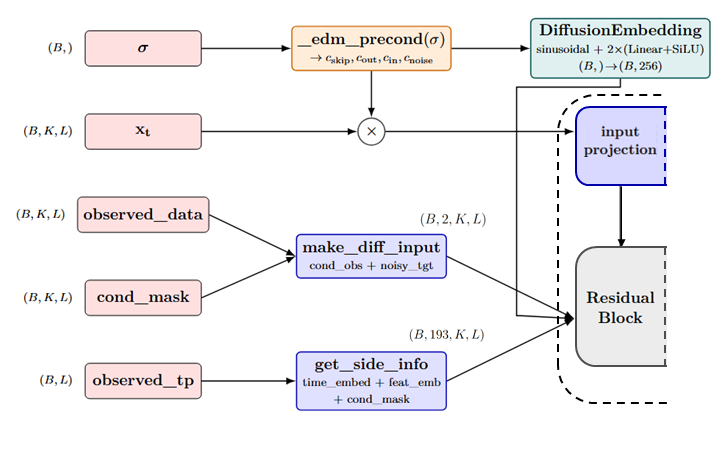
\includegraphics[width=\textwidth]{images/input_drawings.png}
    \caption{Representation of model inputs and how they are feeded into the Denoiser. Input projection and ResidualBlock are those represented in Fig.\ \ref{fig:csdi_overview}.}
    \label{fig:model_input}
  \end{minipage}
  \hfill
  \begin{minipage}[t]{0.28\textwidth}
    \centering
    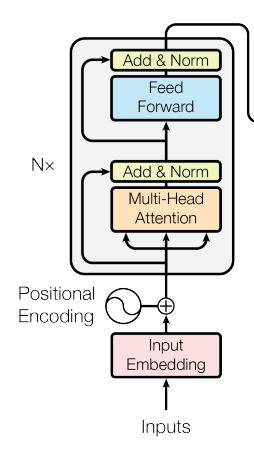
\includegraphics[width=\textwidth]{images/Transformer_architecture_encoder.png}
    \caption{Transformer model architecture for the Encoder. Source: Vaswani et al.\ \cite{vaswani2017attention}.}
    \label{fig:transformer_architecture}
  \end{minipage}
\end{figure}

\textbf{Temporal and feature Transformer layers} \quad A new temporal \((K, L, d)\) and feature \((L, K, d)\) Transformer is initialised per 
residual layer rather than shared across them. Weight sharing would 
constrain all layers to operate at the same level of abstraction, 
limiting the model's ability to build hierarchical representations; 
independent weights allow each layer to specialise. This is consistent 
with the CSDI implementation \cite{tashiro2021csdi}. Multi-head attention 
\cite{vaswani2017attention} allows the model to attend to multiple 
dependency patterns simultaneously within each axis, for instance it could modeled 
short-range trend and longer-range volatility clustering along the temporal axis, or spread relationships along the feature axis. The detailed structure is represented in Fig.\ \ref{fig:transformer_architecture}. 

\textbf{Gated residual blocks} \quad Following the WaveNet structure 
\cite{oord2016wavenet}, each block applies \(\sigma(\cdot) \odot 
\tanh(\cdot)\), where \(\odot\) denotes elementwise multiplication. The 
sigmoid \(\sigma(\cdot)\) acts as the selection gate, producing a value 
in \([0,1]\) that controls how much of the candidate update is passed 
forward. The \(\tanh(\cdot)\) acts as the content filter, producing a 
bounded, signed activation in \([-1,1]\) that encodes \emph{what} 
information to write. Their product suppresses uninformative information 
while preserving significant features. This could be useful for FTS, since Signal-to-Noise Ratio (SNR) is often low and dependents on the regime, training window. 

\textbf{Embeddings} \quad Three embedding mechanisms operate at distinct 
levels of the architecture, each with a well-defined scope. The 
\emph{diffusion-step embedding} (sinusoidal basis projected through two 
linear layers with SiLU activations) encodes \(c_{\text{noise}}(\sigma)\) 
in the EDM phase and the discrete step index \(t\) in the replication 
phase, telling the network the current noise level. The \emph{side information embeddings} 
carry two complementary signals: a time embedding (sinusoidal basis 
followed by a learnable linear projection) encodes the absolute calendar 
position of each time step, allowing the model to associate positions 
with recurring temporal patterns such as month-end or seasonal effects 
that are persistent in the training data; a feature 
embedding is a learned lookup table over channel indices \(\{O, H, L, 
C\}\), giving the model an explicit representation of each channel, enabling channel-specific denoising. Finally, the 
\emph{sinusoidal positional encoding}, following \cite{kim2025diffusion}, 
encodes the relative position of each element within the sequence and is 
injected immediately before each Transformer call, both along the 
temporal and feature axes. Without this the Transformer would be permutation-invariant, which would destroy the temporal order, which is essential for financial return sequences.

\section{Masking strategies}
\label{sec:masking_strategies_ch3} \quad
This work employs two masking strategies: \texttt{unconditional} and \texttt{predict\_close}.

\(\textbf{Phase 1}\quad\) The \texttt{unconditional} setting is used for Phase~1, where \(K=1\) and the model is trained on
univariate log-returns with no conditioning information. The conditioning
mask is \(m^{\text{co}}=0\) everywhere, and the target mask is
\(m^{\text{ta}}=1\) everywhere, so the loss reduces to the
standard denoising objective evaluated on all entries without any side information.

\(\textbf{Phase 2}\quad\) When \(K>1\) we use \texttt{predict\_close} strategy which is a fixed deterministic mask:
\[
    m^{\text{co}}_{k,l} = 1 \quad \text{for } k \in \{O,H,L\}, 
    \qquad
    m^{\text{co}}_{k,l} = 0 \quad \text{for } k = C, 
    \qquad \forall\, l,
\]
and correspondingly:
\[
    m^{\text{ta}}_{k,l} = 0 \quad \text{for } k \in \{O,H,L\}, 
    \qquad
    m^{\text{ta}}_{k,l} = 1 \quad \text{for } k = C, 
    \qquad \forall\, l.
\]
This differs from the random masking used in the original CSDI 
\cite{tashiro2021csdi}, where conditioning and target sets are drawn 
stochastically at each training step. The \texttt{predict\_close} mask 
is closest to CSDI's \emph{test-pattern} strategy, applied at the 
channel level rather than the time-point level, and is consistent with 
the OHLC information structure discussed in 
Sec.~\ref{sec:ohlc_theoretical}: the conditioning set \(\{O,H,L\}\) 
is always observed before \(C\) within a trading session.

As introduced in Sec.~\ref{sec:model_architecture}, the two-channel 
input to the backbone concatenates a signal channel and a mask channel:
\[
    \underbrace{m^{\text{co}} \odot x_0^{\text{co}} + 
    (1-m^{\text{co}}) \odot \bigl(c_{\text{in}}(\sigma)\cdot 
    x_t\bigr)}_{\text{signal channel}}, 
    \qquad
    \underbrace{m^{\text{co}}}_{\text{mask channel}}.
\]
The scaling \(c_{\text{in}}(\sigma)\) is applied only to the noisy 
target entries and not to the clean conditioning observations, since the 
latter carry no noise and no variance drift; rescaling them would destroy 
the conditioning signal. The conditional EDM loss (Eq.~\ref{eq:edm_loss}) 
becomes:
\[
    \mathcal{L}_{\text{cond}}(\theta) = \mathbb{E}_{\sigma,x_0,\epsilon}
    \left[\lambda(\sigma)\,
    \frac{\displaystyle\sum_{k,l} m^{\text{ta}}_{k,l}
    \Bigl(D_\theta\bigl(x_t;\sigma \mid x^{\text{co}}_0, m^{\text{co}}, 
    \tau, f\bigr) - x_0\Bigr)^2_{k,l}}
    {\displaystyle\sum_{k,l} m^{\text{ta}}_{k,l}}
    \right],
\]
where the denominator normalises by the number of active target entries, 
which in the \texttt{predict\_close} setting is fixed and equal to \(L\). 
The additional arguments \(\tau\) (observed time positions 
\texttt{observed\_tp}) and \(f\) (feature indices \texttt{feature\_id}) 
are passed to \(D_\theta\) to construct the side information embeddings, 
consistent with the CSDI implementation.

% The conditioning constraint is enforced at every step of the reverse 
% process. After each Heun update producing a candidate \(\tilde{x}_{i+1}\) 
% for the full \(K\times L\) tensor, the conditioning channels are 
% overwritten with the observed values:
% \[
%     x_{i+1} \xleftarrow[]{} (1-m^{\text{co}}) \odot \text{[update]} 
%     + m^{\text{co}} \odot x_0^{\text{co}},
% \]
% ensuring that the \(O\), \(H\), and \(L\) channels never drift from 
% their observed values during sampling, regardless of what \(D_\theta\) 
% outputs for those positions.

\section{Sampling}

\(\textbf{Phase 1}\quad\) As discussed in Sec.~\ref{sec:scorediffmodels}, the Euler--Maruyama
method performs a first-order discretisation of the reverse SDE, at each
step removing noise while injecting a small stochastic perturbation. 
Because it is first-order, the local truncation error is 
\(\mathcal{O}(h^2)\), and acceptable sample quality typically requires 
hundreds to thousands of steps, implying a high number of neural function 
evaluations (NFEs). Consistently with Song et al.\ \cite{song2021score} 
and CSDI \cite{tashiro2021csdi}, this method is used in the replication 
phase together with the probability flow ODE Eq.\ref{eq:probability_flow} where the learned score \(s_\theta(x_t,t)\) is substituted for the 
intractable \(\nabla_x \log p_t(x_t)\).

\(\textbf{Phase 2}\quad\) In the EDM phase, it was used the Heun second-order
predictor--corrector sampler (Eq.~\ref{eq:edm_sampler}), which 
integrates the probability flow ODE rather than the reverse SDE. The 
corrector step requires twice the number of network evaluations per 
denoising step, but reduces the local truncation error to 
\(\mathcal{O}(h^3)\). Karras et al.\ \cite{karras2022elucidating} report 
that this achieves comparable sample quality to Euler--Maruyama at approximately seven times fewer NFEs.
% As discussed in 
% Sec.~\ref{sec:edm_literature}, the \(\rho\)-power noise schedule 
% concentrates denoising steps at low \(\sigma\), where ODE curvature is 
% highest and discretisation errors have the greatest impact on sample 
% quality.

% The choice of \(\sigma_{\text{max}}\) and \(S_{\text{churn}}\) jointly determines the character of sampling. \(\sigma_{\text{max}}\) sets the noise level at which the reverse process begins, so the prior from which samples are drawn is \(x_N \sim \mathcal{N}(0,\sigma_{\text{max}}^2 I)\); for this prior to be approximately data-free, \(\sigma_{\text{max}}\) must be large enough that the signal-to-noise ratio is negligible. For standardised OHLC log-returns with \(\sigma_{\text{data}} = 1\), values of \(\sigma_{\text{max}} \gg 1\) are required, and setting it too small results in a prior that retains residual data structure, biasing every generated sample. As discussed in Sec.~\ref{sec:edm_literature}, \(S_{\text{churn}}\) governs the amount of stochasticity reinjected per step via the noise inflation \(\hat{\sigma}_i = \sigma_i\sqrt{1+\gamma_i^2}\): a value of \(S_{\text{churn}} = 0\) recovers the deterministic Heun ODE, while positive values allow the sampler to escape discretisation errors by temporarily re-entering a higher-noise regime, at the cost of additional noise injections along each trajectory.

A key advantage of the EDM framework is the decoupling of the sampler
from the training objective: a model trained with the EDM loss can be
evaluated with any compatible ODE or SDE solver without retraining. This
is in contrast to DDPM \cite{ho2020ddpm}, where the sampler and the
noise schedule are tightly coupled to the training procedure.

% \section{Summary}

% This chapter has established the theoretical and architectural foundation 
% of the implemented model. Starting from the financial structure of OHLC 
% data, we motivated the conditioning partition \(\mathcal{C} = \{O,H,L\}\ 
% \to \mathcal{T} = \{C\}\) and acknowledged the structural limitations 
% that the Gaussian diffusion kernel imposes on OHLC consistency. The 
% GBM-inspired VE instantiation was derived from the Black--Scholes 
% framework and its ambiguities with respect to the training data 
% clarified. The EDM preconditioning scheme was interpreted in the context 
% of OHLC log-returns, with particular attention to the consequences of 
% setting \(\sigma_{\text{data}} = 1.0\) on the skip-connection crossover 
% and loss weighting. The CSDI-based architecture was motivated by the 
% global dependency structure of financial time series, and each design 
% choice --- factored attention, gated residual blocks, and the three-level 
% embedding scheme --- was connected to specific properties of the data. 
% Finally, the two masking strategies and the conditional EDM loss were 
% formalised, and the Heun sampler was justified as a more efficient 
% alternative to Euler--Maruyama through its improved truncation error and 
% decoupling from the training objective. The two-phase structure --- 
% replication under Song et al.\ conventions and conditional generation 
% under EDM --- runs consistently through each of these components and 
% provides the basis for the experimental evaluation in Chapter~5.



% %


\chapter{Data and Training Setup}
\label{ch:data_setup}
This section specified the dataset characteristics and training choices. A summary table is made available at Tab.\ref{tab:training_setup}. 
\section{Data}

The dataset follows the source and structure reported by Kim et al.\ \cite{kim2025diffusion}.
Specifically, the list of current S\&P 500 members was taken as the starting universe (as of April 2026), and
tickers with non-standard symbols (e.g., BRK.B, BF.B) were excluded. For each remaining
ticker, the maximum available daily price history was downloaded. The dataset was then
filtered to retain only those stocks whose available history extends at leas 40 years back.
According to the authors:
\begin{quote}
    \emph{This selection criterion ensures that the dataset encompasses diverse market
    regimes, including various boom and bust cycles, thus providing a rich context for
    training the generative model.}
\end{quote}
For each selected stock, daily log-returns were computed as in Eq.~\ref{eq:log_returns},
using the adjusted closing price on day \(t\).

This selection is subject to some limitations. First, survivorship bias: only companies that remained listed for a
period substantially longer than the average tenure in the S\&P 500 index, which is 15 years \cite{slok_apollo_longevity}, are included. The resulting universe therefore may understate the frequency of adverse market events associated with delistings
and corporate failures. The second aspect regards the decimalization process, which was mandated by the Security and Exchange Commission in January 2000 and completed by the 9th of April 2001 \cite{furfine2003decimalization}. Before this period US stock prices were quoted in fractions, specifically 1/16th of a dollar, meaning that the minimum price movement needed to record an effective change in price was 0.0625 dollars. After decimalization this changed to 1 cent. This manifest as 7.1928\% of all returns displaying an exact 0\% daily returns.

\section{Preprocessing}

In Phase 1, only univariate log-returns are used, as defined in Eq.~\ref{eq:log_returns}.
In Phase 2, where conditioning on all four OHLC channels is required, the Open, High,
and Low prices are each expressed as log-returns relative to the previous closing price:
\[
    \hat{O}_t = \log\!\left(\frac{O_t}{C_{t-1}}\right), \qquad
    \hat{H}_t = \log\!\left(\frac{H_t}{C_{t-1}}\right), \qquad
    \hat{L}_t = \log\!\left(\frac{L_t}{C_{t-1}}\right)
\]
This formulation is consistent with the Close log-return defined in Eq.~\ref{eq:log_returns},
expressing all channels relative to the same reference price \(C_{t-1}\).

\(\textbf{Phase~2}\quad\) A per-channel z-score normalisation is then applied independently to each of the four
distribution while standardising it to zero mean and unit variance, so that
\(\sigma_{\text{data}} = 1\) holds by construction and network inputs remain numerically
stable across channels. However, because each channel is scaled by its own standard
deviation, the ordering constraint \(L_t \leq \min(O_t, C_t) \leq \max(O_t, C_t) \leq H_t\),
which holds in price space, is not preserved after normalisation. This is a structural
limitation acknowledged throughout the evaluation.

Four tickers were excluded from the dataset prior to training: BEN, HUBB, NVR, 
and WMB. Each exhibits absolute log-returns exceeding $100\%$, with values 
ranging from $-157\%$ to $+330\%$. Returns below $-100\%$ are theoretically 
inadmissible, because they violate price non-negativity. Such observations are therefore artifacts of the split- and dividend-adjustment procedure described in 
Sec.~\ref{sec:fts_literature}, rather than genuine market events. Exclusion was 
preferred over imputation or smoothing, both of which would introduce their own 
distortions. This choice is consistent with the likely preprocessing of Kim 
et al.~\cite{kim2025diffusion}: after removing these four tickers, the empirical 
distribution aligns more closely with Figure~8 of that paper, 
which is used here as a reference baseline.

\section{Sliding Window Construction}
\label{sec:sliding_window_ch4}

Training sequences are constructed via a sliding window over the full dataset. Two
configurations are used across the two experimental phases:
\begin{itemize}
    \item \textbf{Phase 1, replication:} window length \(L = 2048\) and stride \(s = 400\),
    yielding approximately 5,500 training windows over the full dataset.
    \item \textbf{Phase 2, EDM-CSDI:} window length \(L = 512\) and stride \(s = 100\), yielding approximately 23,000
    training windows cosistent with what described in Ch.~\ref{ch:theoretical_framework}.
\end{itemize}

A window of length \(L = 2048\) spans approximately ten years of daily returns and is
therefore well-suited to capturing long-term trends. However, the temporal Transformer
incurs an \(\mathcal{O}(L^2)\) cost in sequence length, making it computationally
expensive. The shorter \(L = 512\) setting was adopted for Phase 2 due to hardware
constraints imposed by MIG partitioning of the A100 GPU by the High--Performance Computing's university policy. The full memory analysis is given in App.~\ref{app:sec:attention_memory}.

\(\textbf{Phase 1} \quad\) Given the window length the number of non-overlapping windows per ticker is small, making a strict 
train--validation split undesirable. Validation windows were therefore extracted 
by random holdout, consistent with the supposed implementation of Kim 
et al.~\cite{kim2025diffusion}, who are assumed to have either applied a similar random selection or foregone a validation set entirely. Due to the stride, partial overlap between training and validation windows exists.

For the GBM-inspired SDE variant, each window was additionally mean-centred prior 
to training by subtracting the sample mean of the window. This transformation does not conflict with the generative setting, because no forecasting is performed. In addition, any daily log-returns can be easily recovered by \(r_{\tau+k}=C_{\tau+k}-C_{\tau+k-1}\), except for the first element.

\(\textbf{Phase 2}\ \quad \) In order to assess the discriminative power of the conditioning information, validation windows were fully held out: for any ticker whose window was selected for validation, no other window covering the same time range appeared in the training set. This reduces the number of training samples available for learning, however, this effect is mitigated by the larger number of windows available.

% Overlapping windows introduce correlation between adjacent training samples, violating
% the i.i.d.\ batch assumption. This is a standard and accepted approximation in
% deep learning on time series, analogous to patch sampling in image models, but it should
% be noted as a limitation when interpreting training dynamics.

[INTRODUCE WINDOW'S CREATION DIFFERENCE AND include this also in the TABLE for set up; include also sampler for fair comparison]

\section{Training Configuration}
\label{sec:training_config}

This section summarises the most relevant training configuration and design choices;
explicit formulations for the optimiser and learning rate schedule are given in
App.~\ref{app:sec:optim}, and full hyperparameter details in App.~\ref{app:sec:training_config}.

\textbf{Optimizer} \quad The optimiser used throughout is \texttt{AdamW}~\cite{loshchilov2019decoupled},
following the choice of CSDI~\cite{tashiro2021csdi}. It applies weight decay directly
to the parameters rather than through the gradient, preventing the interaction between
$\ell_2$ regularisation and the adaptive scaling of standard Adam. This decoupling results in more consistent regularisation across parameters with different
gradient magnitudes.

\textbf{Learning Rate Scheduler} \quad The learning rate follows cosine
annealing~\cite{loshchilov2017sgdr}, allowing larger updates early in training and progressively smaller updates near
convergence. Reduce-on-Plateau was also evaluated but yielded consistently worse
training dynamics and was not adopted. For Phase~1, $\eta_{\max} = 5 \times 10^{-4}$
and $\eta_{\min} = 1 \times 10^{-6}$; for Phase~2, $\eta_{\max}$ is lowered to
$1 \times 10^{-4}$ to reflect the smaller effective gradient variance under EDM
loss weighting.

\textbf{Model Architecture} \quad  Both phases share the same backbone: 128 \texttt{channels},
6 \texttt{layers}, a 256-dimensional diffusion-step and time embedding, and a
64-dimensional feature embedding, following Kim et al.~\cite{kim2025diffusion}.
This configuration was selected empirically: a 64-channel variant was less expressive,
while a 256-channel variant offered no measurable improvement in generation quality at
substantially higher compute cost.

\textbf{Noise Schedule} \quad The noise hyperparameters differ between phases.
In Phase~1, they define the range of the forward-process noise: VE-style diffusion
uses $\sigma_{\max} = 1$ and $\sigma_{\min} = 0.01$; GBM-style diffusion, operating
on cumulative log-returns, uses $\sigma_{\max} = 10$ and $\sigma_{\min} = 0.1$; and
the VP formulation is parameterised by $\beta_{\max} = 8$ and $\beta_{\min} = 0.01$.
In Phase~2, the EDM log-normal sampling distribution
$\ln\sigma \sim \mathcal{N}(P_{\text{mean}}, P_{\text{std}}^2)$ replaces the
forward-process schedule entirely. The values $P_{\text{mean}} = -1.4$ and
$P_{\text{std}} = 1.6$ were selected via grid search over
$P_{\text{mean}} \in \{-0.8,\,-1.0,\,-1.2,\,-1.4,\,-1.6\}$ and
$P_{\text{std}} \in \{1.0,\,1.2,\,1.4,\,1.6,\,1.8\}$ based on validation loss;
the full ablation is reported in Sec.~\ref{sec:phase2_ablation}.
\textbf{Training parameters.} The batch size is 64 across both phases. Phase~1 trains for the same number of epochs as Kim et al.~\cite{kim2025diffusion}, while Phase~2 uses half that budget, which reflects the hardware constraints and the larger number of available training windows, which increases the number of gradient steps per epoch.

\textbf{Sampling parameters} \quad For Phase~2, $\sigma_{\max}$ and $\sigma_{\min}$ were
selected to cover the support of $\ln\sigma \sim \mathcal{N}(P_{\text{mean}}, P_{\text{std}}^2)$,
requiring $\sigma_{\max} \geq \exp(P_{\text{mean}} + n\,P_{\text{std}})$ for a chosen
coverage multiplier $n$. Three values were tested, $\sigma_{\max} \in \{5,\,7,\,9\}$,
with $\sigma_{\min} = 0.002$ fixed throughout.
\newpage
% Required packages: booktabs, multirow, array
% \usepackage{booktabs, multirow, array}
\begin{table}[htbp]
\centering
\footnotesize
\renewcommand{\arraystretch}{1.35}
\setlength{\tabcolsep}{5pt}
\begin{tabular}{
  >{\itshape}p{2.0cm}
  p{3.0cm}
  p{4.5cm}
  p{4.5cm}
}
\toprule
\normalfont\textbf{Category}
  & \textbf{Parameter}
  & \textbf{Phase 1 \textemdash{} Replication}
  & \textbf{Phase 2 \textemdash{} EDM-CSDI} \\
\midrule
%--- Data & preprocessing ------------------------------------------------
\multirow{5}{2.0cm}{Data \& preprocessing}
  & Channels $K$
  & $K=1$ (close log-return)
  & $K=4$ (OHLC) \\[3pt]
  & Preprocessing
  & Raw close log-return
  & OHLC channels as log-returns relative to $C_{t-1}$;
    per-channel $z$-score normalisation \\[3pt]
  & Conditioning
  & Unconditional;\; $m^{co}=\mathbf{0}$
  & \texttt{predict\_close}: $\{O,H,L\}$ observed,
    $\{C\}$ masked \\[3pt]
  & Window length $L$
  & $2048$ (${\approx}10$ years)
  & $512$ (${\approx}2$ years) \\[3pt]
  & Stride $s$
  & $400$
  & $100$ \\
\midrule
%--- Architecture (shared) -----------------------------------------------
\multirow{5}{2.0cm}{Architecture}                      % FIX 1: 2 -> 5
  & Model channels
  & \multicolumn{2}{c}{$128$} \\[3pt]
  & Layers
  & \multicolumn{2}{c}{$6$} \\[3pt]
  & Diffusion emb.
  & \multicolumn{2}{c}{$256$} \\[3pt]              % FIX 3: added [3pt]
  & Time emb.
  & \multicolumn{2}{c}{$128$} \\[3pt]              % FIX 3: added [3pt]
  & Feature emb.
  & \multicolumn{2}{c}{$64$} \\                    % FIX 2: added \\
\midrule
%--- Noise schedule ------------------------------------------------------
\multirow{3}{2.0cm}{Noise schedule}
  & $\sigma_{\max}$ / $\sigma_{\min}$
  & VE:\;$\sigma_{\max}{=}1,\;\sigma_{\min}{=}0.01$;\;
    GBM:\;$\sigma_{\max}{=}10,\;\sigma_{\min}{=}0.1$
  & \textemdash \\[3pt]
  & $\beta_{\max}$ / $\beta_{\min}$
  & VP:\;$\beta_{\max}{=}8,\;\beta_{\min}{=}0.01$
  & \textemdash \\[3pt]
  & $P_{\text{mean}}$ / $P_{\text{std}}$
  & \textemdash
  & $P_{\text{mean}}{=}{-1.4},\;P_{\text{std}}{=}1.6$ \\
\midrule
%--- Training ------------------------------------------------------------
\multirow{4}{2.0cm}{Training}                          % FIX 4: 3 -> 4
  & LR schedule
  & \multicolumn{2}{c}{cosine annealing} \\[3pt]
  & $\eta_{\max}$ / $\eta_{\min}$
  & $5\!\times\!10^{-4}$ / $1\!\times\!10^{-6}$
  & $1\!\times\!10^{-4}$ / $1\!\times\!10^{-6}$ \\[3pt]
  & Epoch
  & $1000$
  & $500$ \\
  & Batch size
  & \multicolumn{2}{c}{$64$} \\[3pt]
  & Optimizer
  & \multicolumn{2}{c}{\texttt{AdamW}} \\
  & Early-stopping
  & \textemdash
  & validation-loss; 200 epochs\\
\midrule

\multirow{3}{2.0cm}{Sampling}
  & Method
  & \makecell[l]{Euler--Maruyama SDE\\Probability-flow ODE}
  & \makecell[l]{Heun ODE\\Stochastic Heun SDE} \\
  & $\sigma_{\max}$ / $\sigma_{\min}$
  & from \emph{Noise schedule}
  & $\sigma_{\max}=7.0$, $\sigma_{\min}=0.002$\\
\bottomrule
\end{tabular}
\caption{Training setup for Phase~1 (replication of Kim et al.\ \cite{kim2025diffusion})
and Phase~2 (EDM-CSDI). Parameters shared across both phases appear in merged cells. \emph{emb.} is short for embeddings.}
\label{tab:training_setup}
\end{table}

\chapter{Evaluation Methodology}
\label{ch:evaluation_methodology}
This chapter presents the evaluation methodology applied to both unconditional and
conditional generated data. Multiple metrics are used to assess distributional similarity,
moment reproduction, path-wise behaviour, and conditional predictive quality, combining
quantitative metrics with visual insights.

\section{Distributional Similarity}

To assess the similarity between the real and generated data distributions, two
complementary metrics are reported: the Wasserstein distance \cite{arjovsky2017wasserstein},
which captures global distributional shifts, and the Kolmogorov--Smirnov (KS) test
\cite{massey1951kolmogorov}, which provides a nonparametric hypothesis test for
distributional differences. Both metrics are computed on the log-return datasets
\(\mathcal{D}_{\text{train}}\) and \(\mathcal{D}_{\text{gen}}\).

\textbf{Kolmogorov--Smirnov} \quad The KS statistic measures the maximum distance between
the empirical cumulative distribution functions of two samples. Given two empirical
cumulative distributions \(F(x)\) and \(G(x)\), it is defined as:
\[
    D_{\text{KS}} = \sup_x |F(x) - G(x)|
\]
where \(\sup_x\) denotes the supremum over all values of \(x\). The KS test is
advantageously nonparametric and sensitive to both location and shape differences;
however, its maximum deviation is dominated by the bulk of the distribution and is
relatively insensitive to tail discrepancies.

\textbf{Wasserstein Distance} \quad The Wasserstein distance measures the minimal effort
required to transform one distribution into another. For two cumulative distributions
\(F(x)\) and \(G(x)\), it is defined as:
\[
    W_1(F, G) = \int_{-\infty}^{\infty} |F(x) - G(x)|\, dx
\]
Unlike the KS statistic, which reports only the maximum deviation, \(W_1\) integrates
the discrepancy across the entire support, providing a global measure of distributional
mismatch.

\section{Aggregate Statistics}

To obtain a more comprehensive view of generative quality, the pathwise mean, variance,
skewness, and kurtosis are computed for each window in \(\mathcal{D}_{\text{train}}\) and
\(\mathcal{D}_{\text{gen}}\). Scalar metrics such as KS and \(W_1\) flatten temporal
structure; pathwise higher-order moments instead provide direct evidence of whether the
model reproduces non-Gaussian behaviour and the stylized facts of financial time series,
with particular attention to skewness and excess kurtosis. The latter must be interpreted with caution, since, as discussed in Sec.\ \ref{sec:fts_literature}, the fourth moment is likely unbounded for FTS. Hence, even if computationally finite on a limited dataset, it may be infinite for the true underlying population.

\section{Visualizations}
Complementary with the statistics we plotted different sets of graphs.

\textbf{Quantile--Quantile (QQ) Plots} \quad Quantile comparison between pooled generated and real returns are useful to check whether a model who can match the bulk if it still misses the tails. By plotting quantiles of \(D_{\text{gen}}\)\ again the quantiles of \(D_{\text{train}}\).

\textbf{ECDF Plots} \quad It is a visual complement to the KS test. Plot the Empirical Cumulative Distribution Functions \(\hat{F}_{\text{gen}}\) and \(\hat{F}_{\text{data}}\) together with the KS gap marked. This makes the KS statistic more interpretable.

\textbf{Unnormalized Paths} \quad Invert the normalisation to recover approximate price-level trajectories. This serves primarily as a sanity and plausibility check of the model's ability to generate coherent price levels, where ``unnormalize'' denotes applying the inverse of the global z-score.

\section{Financial Time Series Evaluation}
For financial time series, a set of tools is used to compute the tail distribution,
the autocorrelation function (ACF), the leverage effect, and a power-law tail
exponent \(\alpha\). These metrics are implemented following the functions provided
in \cite{stakahashy_fingan}, which was also adopted by Kim et al.\
\cite{kim2025diffusion}, enabling a direct comparison with their results. For
consistency, the power-law coefficient is computed using the same Python package:
\texttt{powerlaw} by Alstott et al.\ \cite{alstott2014powerlaw}. The definitions of the tail distribution, \(\alpha\),
volatility clustering, and the leverage effect are provided in
Sec.\ \ref{sec:fts_literature}. Following Kim et al.\ \cite{kim2025diffusion}, the heavy-tail diagnostic and the exponent \(\alpha\) are computed on the positive (right) tail only.

Following FinGAN\ \cite{stakahashy_fingan} and Kim et al.\ \cite{kim2025diffusion}, in Phase~1 the maximum lag for the leverage effect is set to 100 and for volatility clustering to 1000. In Phase~2, the maximum lag for volatility clustering is reduced to 256 for estimation stability. The ACF at lag \(k\) is estimated over \(L - k\) observation pairs; for a window of length \(L = 512\), lags approaching \(L\) leave too few pairs to produce reliable estimates, rendering a maximum lag of 512 impractical. Setting the upper bound to \(L/2 = 256\) ensures that at least half the window's values contributes to each estimate.


\section{Conditional Evaluation}
When evaluating the conditional generation we are evaluating the quality of the conditional generation by focusing on CRPS (Continuous Rank Probability Score) and interval coverage.

\textbf{CRPS} \quad This metrics is measured as:
\[
\text{CRPS}(\hat{F}, y) = \mathbb{E}_{\hat{F}} \left[|X - y|\right] - \tfrac{1}{2}\,\mathbb{E}_{\hat{F}}\left[|X - X'|\right]
\]

where \(X,X'\) are independent draws from the predictive ensemble \(\hat{F}\) and \(y\) is the observed Close. CRPS \cite{matheson1976scoring} is a proper scoring rule: it penalises inaccuracy 
(the first term) and rewards spread (the second term lowers CRPS as ensemble 
diversity grows). It reduces to MAE when the distribution collapses to a point forecast, so it can be interpreted as a calibration-adjusted MAE, where \(0 \le \text{CRPS}\le\text{MAE}\) (proof in Sec.\ \ref{app:sec:crps_bounds}). This score is also used in CSDI \cite{tashiro2021csdi}. Nevertheless, a raw CRPS value is difficult to interpret in isolation, so it was constructed a \emph{climatology} baseline whose ensemble is formed by drawing, with replacement, from the full pool of observed Close log-returns, ignoring the OHL conditioning. A second baseline fits an OLS regression of Close on the same-day Open, High, and Low log-returns, with its ensemble formed by adding bootstrapped residuals to the OLS point forecast. Relative skill is summarised by the CRPS skill score $\text{SS}_{\text{CRPS}} = 1 - \overline{\text{CRPS}}_{\text{model}} / \overline{\text{CRPS}}_{\text{baseline}}$, where $1$ is perfect, $0$ means no improvement over the uninformative baseline.

\textbf{Interval Coverage} \quad This metrics is measure for nominal coverage levels, \(1-\alpha \in \{0.5,0.8,0.9,0.95,0.99\}\). Once defined the nominal level investigated the empirical coverage is:
\[
\text{coverage}_{1-\alpha} = \frac{1}{N} \sum_{t=1}^{L} \sum_{n=1}^{N_t} \mathbf{1}\left[y_{n,t} \in \bigl[q_{\alpha/2}(n,t),\; q_{1-\alpha/2}(n,t)\bigr]\right]
\]
where \(q\) are ensemble quantiles, which means they are quantiles computed from the set of multiple forecasts the model produces for the same target value, or set of conditioning information. A well-calibrated model has the empirical value approximately identical to nominal. Positive gap means underconfidence (intervals too wide), negative gap means overconfidence (intervals too narrow).



\chapter{Experiments and results}
Another problem to consider is fully held-out windows.
\begin{itemize}
    \item Lower error for smaller ts between linear and exponential because of higher discriminative power
\end{itemize}

1. Phase 1, 2048/400 replication
2. Phase 2, expansion to edm 512/100 performance and comparison with baseline models
3. Further expansion and evaluation of EDM models (against baseline possibly)

\section{Introduction}
In this chapter we will analyse the experiments conducted and the results yielded. Before proceeding it is important to underline the two core questions we are trying to answer here:
\begin{itemize}
    \item Are we able to replicate the results obtained by Kim et al. \cite{kim2025diffusion} and to which extent?
    \item Does the embedding into EDM and the introduction of conditional information improved models' performance and ability to replicate true FTS distribution?
\end{itemize}
\section{Phase 1}
For phase 1 the settings are available at Tab.\ref{tab:training_setup}. On top of these, models were trained for 1000 epochs, similarly to Kim et al. \cite{kim2025diffusion} with batch size of 64. The sampling technique is probability flow ODE, which empirically have been show produing more reliable and replicable results.


[INCLUDE IMAGES THAT SHOW FTS AND RELEVANT OTHER GRAPHS OR TABLE]

General structure:
* Aggregate statistics
* distributional information
* Stylized facts + alpha
* path illustration

For conditional add also:
* CRPS
* Interval Coverage

\section{Phase 2}
In this section it is conducted a comparative study of EDM alongside previous implementation. Specifically, we evaluate the conditioning. In order to have a fair assessment, the models analysed in Phase 1 were re-trained with \(L=512\) and \(stride=100\) and the same Heun's ODE sampler was used.

[Remember of the different window-training instantializationhttps://www.trekkinglecco.com/sentiero-viandante/]


\chapter{Discussion}
\begin{itemize}
    \item Masking: one of the key advantages of CSDI is to use randmask, so that it can learn the global and local structure instead of being always conditional (like Classifier Free Guidance) -> Future work expand on this
    \item \(\sigma_{\text{data}}\) ablation
    \item exploration of other \(c_{noise}\)
    \item We did not explore the contribution of EDM preconditioning and conditional information alone, meaning that it is impossible to discer which contributes what to improving prediction (if at all)
    \item no ablation was done on embeddings dimensions
    \item This makes \(t\)-EDM a possible future extension of the EDM--CSDI framework considered in this thesis, since it preserves much of the EDM structure while changing the tail behaviour of the noising distribution.
    \item Baseline comparison with other Deep learning models
\end{itemize}

here are some \textbf{Future works}
\begin{itemize}
    \item expan into the heavy tail diffusion model with focus on that literature
    \item learnable skip connection
    \item testing the two components individually: conditional information and preconditioning EDM
    \item add learnable parameter for PE (relative)
\end{itemize}

\chapter{Conclusion}

Your conclusion here.

\bibliographystyle{plain}
\bibliography{references}

% \appendix
% \chapter{Mathematical Foundations}
\label{app:math_foundations}

This appendix provides expanded mathematical background for the classical models
discussed in Section~2.2 and the stochastic framework underlying them. It is
intended as a self-contained reference that deepens the treatment of Brownian
motion, It\^{o}'s Lemma, the Poisson process, and the structural limitations of
GARCH and Merton's jump-diffusion model, without repeating the main exposition.
Throughout this appendix, $t$ denotes calendar time; when referencing
Eq.~(\ref{eq:blackscholes}) from the main text, $t$ plays the role of $\tau$.

\section{Brownian Motion}
\label{app:sec:bm}

Brownian motion is the continuous-time stochastic process that underlies both
the white-noise innovations of GARCH and the diffusion component of the GBM in
Eq.~(\ref{eq:blackscholes}). It was first formally constructed by Wiener (1923)
and is therefore also called the \textit{Wiener process}; the name
\textit{Brownian motion} traces back to the botanist Robert Brown, who in 1827
observed the erratic movement of pollen particles suspended in water, a
phenomenon later explained by Einstein (1905) as the effect of random molecular
collisions.\\

\textbf{Definition.} A stochastic process $\{W_t\}_{t \geq 0}$ defined on a
probability space $(\Omega, \mathcal{F}, \mathbb{P})$ is called a
\textit{standard Brownian motion} if it satisfies the following four properties:
\begin{enumerate}
    \item \textit{Initialisation}: $W_0 = 0$ almost surely.
    \item \textit{Independent increments}: for any $0 \leq t_0 < t_1 < \cdots <
    t_n$, the increments $W_{t_1} - W_{t_0},\, W_{t_2} - W_{t_1},\, \ldots,\,
    W_{t_n} - W_{t_{n-1}}$ are mutually independent random variables.
    \item \textit{Stationary Gaussian increments}: for any $0 \leq s < t$,
    \begin{equation}
        \label{eq:bm_increment}
        W_t - W_s \;\sim\; \mathcal{N}(0,\, t - s).
    \end{equation}
    \item \textit{Continuous paths}: the map $t \mapsto W_t$ is almost surely
    continuous.
\end{enumerate}

These four axioms are minimal and mutually consistent: any two of them, together
with mild regularity, imply the others \cite{oksendal2003stochastic}.\\

\textbf{Intuition: the limit of a random walk.} Brownian motion can be understood
as the continuous-time limit of a symmetric random walk. Partition $[0, T]$ into
$N$ steps of length $\Delta t = T/N$, and at each step $k$ add $+\sqrt{\Delta t}$
or $-\sqrt{\Delta t}$ with equal probability. The position after $k$ steps is
$Z_k = \sum_{i=1}^k \xi_i \sqrt{\Delta t}$ where $\xi_i \in \{-1, +1\}$ with
equal probability. The variance of $Z_k$ is $k \cdot \Delta t$, which remains
finite as $N \to \infty$ provided $\Delta t = T/N$. By the Central Limit
Theorem, $Z_{\lfloor tN \rfloor}$ converges in distribution to $W_t \sim
\mathcal{N}(0, t)$. The $\sqrt{\Delta t}$ scaling is not optional: scaling by
$\Delta t$ would collapse all increments to zero, while scaling by a constant
would produce infinite variance. This is the only scaling that gives a
well-defined non-degenerate continuous-time limit.

\subsection{Key Statistical Properties}

Setting $s = 0$ in property~3, we immediately obtain:
\[
    \mathbb{E}[W_t] = 0, \qquad \operatorname{Var}(W_t) = t, \qquad
    W_t \sim \mathcal{N}(0,\, t).
\]
The variance grows linearly in time: uncertainty accumulates at rate $\sqrt{t}$,
not $t$. This sub-linear growth is the signature of diffusion and contrasts with
a deterministic path (variance 0) or with a purely random variable with no time
structure.\\

\textbf{Covariance and correlation.} For $0 \leq s \leq t$, write
$W_t = W_s + (W_t - W_s)$. Since $W_t - W_s$ is independent of $W_s$ (property~2)
and has mean zero:
\begin{align*}
    \operatorname{Cov}(W_s, W_t)
    &= \operatorname{Cov}\bigl(W_s,\; W_s + (W_t - W_s)\bigr) \\
    &= \operatorname{Var}(W_s) + \underbrace{\operatorname{Cov}(W_s,\,
       W_t - W_s)}_{=\,0}
    \;=\; s \;=\; \min(s, t).
\end{align*}
Consequently $\operatorname{Corr}(W_s, W_t) = \sqrt{s/t}$ for $s \leq t$.
Two observations far apart in time are weakly correlated; the process has no
long-range memory beyond the information contained in its current value, a
property formalised next.\\

\textbf{Markov property.} The future distribution of $W_t$ given all past
information $\mathcal{F}_s = \sigma(W_u : u \leq s)$ depends on the past only
through the current value $W_s$:
\[
    P(W_t \in A \mid \mathcal{F}_s) = P(W_t \in A \mid W_s), \qquad s \leq t.
\]
This follows from independent increments: $W_t - W_s \sim \mathcal{N}(0, t-s)$
is independent of $\mathcal{F}_s$, so knowing the full path up to $s$ adds
nothing beyond knowing $W_s$. Economically, this says that the noise driving
asset prices has no exploitable history: past increments of $W$ carry no
information about future ones.\\

\textbf{Martingale property.} With respect to $\{\mathcal{F}_t\}$, $W_t$ is a
martingale:
\[
    \mathbb{E}[W_t \mid \mathcal{F}_s] = W_s, \qquad s \leq t.
\]
Proof: $\mathbb{E}[W_t \mid \mathcal{F}_s] = \mathbb{E}[W_s + (W_t - W_s)
\mid \mathcal{F}_s] = W_s + \mathbb{E}[W_t - W_s] = W_s$, using independence
and zero mean of the increment. The martingale property encodes the absence of
predictable drift in the noise: knowing the path up to $s$, the best prediction
of $W_t$ is simply $W_s$, with no systematic upward or downward tendency.

\subsection{Quadratic Variation and Non-Differentiability}

A central and counter-intuitive property of BM is that its paths are almost
surely continuous yet nowhere differentiable. This is not a pathological edge
case: it holds with probability one and is intimately connected to the
\textit{quadratic variation} of the process.\\

\textbf{Quadratic variation.} For a partition $\Pi = \{0 = t_0 < t_1 < \cdots
< t_n = t\}$ with mesh $\|\Pi\| = \max_i(t_{i+1} - t_i)$, the quadratic
variation of $W$ over $[0, t]$ is:
\begin{equation}
    \label{eq:quadratic_variation}
    [W]_t \;=\; \lim_{\|\Pi\| \to 0}\; \sum_{i=0}^{n-1}(W_{t_{i+1}} -
    W_{t_i})^2 \;=\; t,
\end{equation}
where the limit holds in $L^2$. To verify this, write $\delta_i = W_{t_{i+1}}
- W_{t_i}$:
\[
    \mathbb{E}\!\left[\sum_i \delta_i^2\right] = \sum_i(t_{i+1} - t_i) = t,
\]
\[
    \operatorname{Var}\!\left[\sum_i \delta_i^2\right]
    = \sum_i \operatorname{Var}(\delta_i^2)
    = \sum_i 2(t_{i+1} - t_i)^2
    \leq 2\|\Pi\|\sum_i(t_{i+1} - t_i)
    = 2\|\Pi\|\, t \;\xrightarrow{\|\Pi\|\to 0}\; 0.
\]
The mean is $t$ and the variance vanishes, so the sum converges in $L^2$ to $t$,
establishing Eq.~(\ref{eq:quadratic_variation}). This result is written
compactly in It\^{o} calculus as the \textit{multiplication rules}:
\begin{equation}
    \label{eq:ito_product_rules}
    (dW_t)^2 = dt, \qquad dW_t\cdot dt = 0, \qquad (dt)^2 = 0.
\end{equation}

For comparison, any deterministic differentiable function $f$ has zero quadratic
variation: its increments are $O(\Delta t)$ so their squares sum to
$O(\|\Pi\|) \to 0$. The non-zero quadratic variation of BM means that it
oscillates so violently on small time scales that the sum of squared increments
is macroscopically significant. Two direct consequences follow:
\begin{itemize}
    \item \textit{Infinite total variation}: $\sum_i |\delta_i| \to \infty$ as
    $\|\Pi\| \to 0$ almost surely. BM paths cannot be approximated by smooth
    curves in the sense of bounded variation.
    \item \textit{Nowhere differentiability}: if $W$ were differentiable at
    some point $t$, then $|\delta_i| = O(\Delta t)$, giving $\sum_i \delta_i^2
    = O(\|\Pi\|) \to 0$, contradicting $[W]_t = t > 0$. Hence no derivative
    exists almost surely at any point.
\end{itemize}

Financially, nowhere differentiability means that instantaneous
``speed'' $dW_t/dt$ does not exist: price changes driven by BM are inherently
irregular at every time scale and carry no predictable directional momentum from
one instant to the next.

\section{It\^{o}'s Lemma and the Black-Scholes Model}
\label{app:sec:ito}

Ordinary calculus provides the chain rule: if $f$ is smooth and $x(t)$ is
differentiable, then $df = f'(x)\,dx$. Because BM paths are not differentiable,
this rule fails when $x$ is driven by a Brownian motion. The extra term in the
quadratic variation, $(dW_t)^2 = dt \neq 0$, means that the second-order
contribution in the Taylor expansion is of order $dt$ and cannot be discarded.
It\^{o}'s Lemma provides the correct generalisation.

\subsection{Statement and Heuristic Proof}

Let $\{X_t\}$ be an It\^{o} process satisfying:
\[
    dX_t = a_t\, dt + b_t\, dW_t,
\]
where $a_t$ (the drift) and $b_t$ (the diffusion coefficient) are adapted
stochastic processes satisfying standard integrability conditions
\cite{oksendal2003stochastic}. Let $f(t, x)$ be a function that is once
continuously differentiable in $t$ and twice continuously differentiable in $x$.
Then:
\begin{equation}
    \label{eq:ito_lemma}
    df(t, X_t) = \left(\frac{\partial f}{\partial t}
    + a_t\, \frac{\partial f}{\partial x}
    + \frac{1}{2}\, b_t^2\,
    \frac{\partial^2 f}{\partial x^2}\right)\! dt
    + b_t\, \frac{\partial f}{\partial x}\, dW_t.
\end{equation}

The term $\frac{1}{2} b_t^2 \frac{\partial^2 f}{\partial x^2}\, dt$ is the
\textbf{It\^{o} correction}. It is absent in ordinary calculus and arises
because the stochastic increment has a non-negligible second-order contribution.
In vector form, for a function $f(t, \mathbf{X}_t)$ of a
multi-dimensional It\^{o} process $d\mathbf{X}_t = \mathbf{a}_t\,dt +
\mathbf{B}_t\,d\mathbf{W}_t$, the correction becomes
$\frac{1}{2}\operatorname{tr}\!\left(\mathbf{B}_t\mathbf{B}_t^{\top}
\nabla^2 f\right)dt$, but the one-dimensional case suffices for the
applications in Chapter~2.\\

\textit{Heuristic derivation.} Expand $f(t + dt, X_{t+dt})$ by Taylor's theorem
to second order in $dX_t$ and first order in $dt$:
\[
    df = \frac{\partial f}{\partial t}\, dt
       + \frac{\partial f}{\partial x}\, dX_t
       + \frac{1}{2}\frac{\partial^2 f}{\partial x^2}(dX_t)^2
       + \cdots
\]
Substitute $dX_t = a_t\, dt + b_t\, dW_t$ and expand $(dX_t)^2$:
\[
    (dX_t)^2 = a_t^2(dt)^2 + 2a_t b_t\, dt\, dW_t + b_t^2(dW_t)^2.
\]
Applying the rules in Eq.~(\ref{eq:ito_product_rules}):
\[
    (dX_t)^2 = b_t^2\, dt.
\]
The cross term $dt\,dW_t$ and the higher-order term $(dt)^2$ vanish. Collecting
the surviving contributions:
\[
    df = \frac{\partial f}{\partial t}\, dt
       + \frac{\partial f}{\partial x}(a_t\, dt + b_t\, dW_t)
       + \frac{1}{2}\frac{\partial^2 f}{\partial x^2}\, b_t^2\, dt,
\]
which rearranges to Eq.~(\ref{eq:ito_lemma}). The rigorous proof replaces
this Taylor expansion argument with an $L^2$ limit over sequences of
partitions \cite{oksendal2003stochastic}; the intuition is identical.

\subsection{Proof of the Black-Scholes Price Equation}

Chapter~2 states that applying It\^{o}'s Lemma to $\log S_t$ under GBM
(Eq.~\ref{eq:blackscholes}) yields the log-normal price formula. We derive
this in full here. The GBM is the It\^{o} process with drift coefficient
$a_t = \mu S_t$ and diffusion coefficient $b_t = \nu S_t$:
\[
    dS_t = \mu\, S_t\, dt + \nu\, S_t\, dW_t.
\]
Apply It\^{o}'s Lemma (Eq.~\ref{eq:ito_lemma}) to $f(S_t) = \log S_t$:
\[
    \frac{\partial f}{\partial t} = 0, \qquad
    \frac{\partial f}{\partial S} = \frac{1}{S_t}, \qquad
    \frac{\partial^2 f}{\partial S^2} = -\frac{1}{S_t^2}.
\]
Substituting $a_t = \mu S_t$ and $b_t = \nu S_t$:
\begin{align*}
    d(\log S_t)
    &= \left(0 + \mu S_t \cdot \frac{1}{S_t}
       + \frac{1}{2}(\nu S_t)^2 \cdot \left(-\frac{1}{S_t^2}\right)\right)\! dt
       + \nu S_t \cdot \frac{1}{S_t}\, dW_t \\
    &= \left(\mu - \frac{1}{2}\nu^2\right)\! dt + \nu\, dW_t.
\end{align*}
This is a Brownian motion with constant drift $\mu - \frac{1}{2}\nu^2$ and
constant diffusion coefficient $\nu$. Integrating over $[0, t]$:
\[
    \log S_t - \log S_0
    = \left(\mu - \frac{1}{2}\nu^2\right)t + \nu W_t,
\]
and exponentiating:
\begin{equation}
    \label{eq:gbm_solution_app}
    S_t = S_0 \exp\!\left[\left(\mu - \frac{1}{2}\nu^2\right)t
          + \nu W_t\right].
\end{equation}
Since $W_t \sim \mathcal{N}(0, t)$, the log-return over $[0, t]$ satisfies:
\begin{equation}
    \label{eq:lognormal_returns_app}
    \log\!\left(\frac{S_t}{S_0}\right)
    \;\sim\; \mathcal{N}\!\left(\left(\mu - \frac{1}{2}\nu^2\right)t,\;
    \nu^2 t\right).
\end{equation}
Log-returns are normally distributed with mean proportional to $t$ and variance
proportional to $t$, confirming the statement in Section~2.2 and the foundation
of the Black--Scholes option pricing model \cite{black1973pricing}.\\

\textbf{Interpreting the It\^{o} correction.} The term $-\frac{1}{2}\nu^2$ is
not an approximation error: it is the exact price of the convexity of the
exponential function. Because $x \mapsto e^x$ is convex, Jensen's inequality
gives $\mathbb{E}[e^X] \geq e^{\mathbb{E}[X]}$ for any random variable $X$. For
$X = (\mu - \frac{1}{2}\nu^2)t + \nu W_t$, we have $\mathbb{E}[X] = (\mu -
\frac{1}{2}\nu^2)t$ and $\mathbb{E}[e^X] = e^{\mu t}$; indeed:
\[
    \mathbb{E}[S_t] = S_0\, e^{(\mu - \frac{1}{2}\nu^2)t}\,
    \mathbb{E}\!\left[e^{\nu W_t}\right]
    = S_0\, e^{(\mu - \frac{1}{2}\nu^2)t}\cdot e^{\frac{1}{2}\nu^2 t}
    = S_0\, e^{\mu t},
\]
where $\mathbb{E}[e^{\nu W_t}] = e^{\frac{1}{2}\nu^2 t}$ is the moment
generating function of the Gaussian. The correction ensures that the arithmetic
expected return of prices is $\mu$ (as specified in the SDE), while the
geometric mean return is the lower quantity $\mu - \frac{1}{2}\nu^2$. This
gap, $\frac{1}{2}\nu^2$, is called \textit{variance drag}: higher volatility
reduces the realised compound return even holding the instantaneous drift fixed.
Without the It\^{o} correction, applying the classical chain rule would give
$d(\log S_t) = \mu\, dt + \nu\, dW_t$, implying $\log(S_t/S_0) \sim
\mathcal{N}(\mu t, \nu^2 t)$ and therefore $\mathbb{E}[S_t] = S_0
e^{\mu t + \frac{1}{2}\nu^2 t}$, which contradicts $\mathbb{E}[S_t] = S_0
e^{\mu t}$ derived directly from the SDE.

\section{Poisson Process and Merton's Jump-Diffusion Model}
\label{app:sec:poisson_merton}

The Poisson process is the canonical model for events that arrive randomly,
infrequently, and with no predictable timing — in the financial context, sudden
discontinuous jumps in asset prices caused by earnings surprises, credit events,
regulatory changes, or macroeconomic shocks. It complements Brownian motion by
introducing discontinuous sample paths, allowing the model to generate
large price moves instantaneously rather than through accumulated small
increments.

\subsection{The Poisson Process}

\textbf{Definition.} A stochastic process $\{P_t\}_{t \geq 0}$ taking values in
$\mathbb{N}_0 = \{0, 1, 2, \ldots\}$ is a \textit{Poisson process with intensity}
$\lambda > 0$ if:
\begin{enumerate}
    \item $P_0 = 0$ almost surely.
    \item Independent increments: for any $0 \leq t_0 < t_1 < \cdots < t_n$,
    the increments $P_{t_1} - P_{t_0},\, \ldots,\, P_{t_n} - P_{t_{n-1}}$ are
    mutually independent.
    \item Stationary Poisson increments: for any $0 \leq s < t$,
    \begin{equation}
        \label{eq:poisson_increment}
        P_t - P_s \;\sim\; \operatorname{Poisson}(\lambda(t - s)),
    \end{equation}
    i.e., $P(P_t - P_s = k) = \frac{e^{-\lambda(t-s)}[\lambda(t-s)]^k}{k!}$
    for $k \in \mathbb{N}_0$.
    \item At most one event per instant: $P(P_{t+h} - P_t \geq 2) = o(h)$
    as $h \to 0^+$.
\end{enumerate}

The process $P_t$ counts the number of jumps that have occurred by time $t$.
From Eq.~(\ref{eq:poisson_increment}):
\[
    \mathbb{E}[P_t] = \lambda t, \qquad \operatorname{Var}(P_t) = \lambda t.
\]
The equality of mean and variance is the defining property of the Poisson
distribution: the intensity $\lambda$ simultaneously controls the average
jump rate and the variability of the jump count. A small $\lambda$ means
rare, widely-spaced jumps; a large $\lambda$ means frequent ones.\\

\textbf{Inter-arrival times.} The waiting times between consecutive jumps
$\tau_1, \tau_2, \ldots$ are independent and exponentially distributed with
mean $1/\lambda$:
\[
    \tau_k \;\sim\; \operatorname{Exp}(\lambda), \qquad
    P(\tau_k > s) = e^{-\lambda s}.
\]
The memoryless property of the exponential distribution mirrors the independent
increments of $P_t$: the time until the next jump does not depend on how long
one has already waited. This is a deliberate modelling choice; in reality, jump
arrivals in markets are not memoryless (see Section~\ref{app:sec:limitations}).\\

\textbf{Martingale structure.} The \textit{compensated Poisson process}
$\widetilde{P}_t = P_t - \lambda t$ is a martingale with zero mean and
$\operatorname{Var}(\widetilde{P}_t) = \lambda t$. The deterministic term
$\lambda t$ is the \textit{compensator}: it removes the upward drift of $P_t$,
playing the same role for the Poisson process that zero mean plays for $W_t$.

\subsection{Merton's Jump-Diffusion Model}

Merton \cite{merton1976option} extended the GBM (Eq.~\ref{eq:blackscholes}) by
superimposing a compound Poisson jump component onto the continuous diffusion:
\begin{equation}
    \label{eq:merton_sde_app}
    dS_t = \mu\, S_t\, dt + \nu\, S_t\, dW_t + S_{t^-}(J - 1)\, dP_t.
\end{equation}
The three terms have distinct roles:
\begin{itemize}
    \item $\mu\, S_t\, dt$: the continuous expected-return drift, as in GBM.
    \item $\nu\, S_t\, dW_t$: the diffusion noise, modelling continuous
    day-to-day fluctuations with constant volatility $\nu > 0$.
    \item $S_{t^-}(J - 1)\, dP_t$: the jump term. Here $S_{t^-}$ denotes
    the price immediately \textit{before} a possible jump at time $t$,
    $P_t$ is a Poisson process with intensity $\lambda$ independent of $W_t$,
    and $J > 0$ is a random jump multiplier, i.i.d.\ across jump events and
    independent of both $W_t$ and $P_t$. When $dP_t = 1$, the price jumps
    from $S_{t^-}$ to $S_{t^-} \cdot J$; when $dP_t = 0$, the jump term
    vanishes.
\end{itemize}

\textbf{Distribution of the jump multiplier.} As discussed in Section~2.2, the
log-return distribution under Merton's model is a Poisson-weighted mixture of
Gaussians. This result requires $\log J$ to be normally distributed; consistent
with Merton's (1976) original formulation, $J$ is therefore \textit{log-normally}
distributed:
\begin{equation}
    \label{eq:jump_lognormal_app}
    \log J \;\sim\; \mathcal{N}(\mu_j,\, \sigma_J^2).
\end{equation}
The parameter $\mu_j$ is the mean log-jump size: $\mu_j > 0$ corresponds to
jumps that are on average upward, $\mu_j < 0$ to downward jumps, and $\mu_j = 0$
to symmetric jumps. The parameter $\sigma_J^2$ controls the dispersion of jump
sizes; larger $\sigma_J$ produces a wider range of jump magnitudes and heavier
tails. The log-normal specification also guarantees $J > 0$, ensuring that
prices remain positive after any jump.

\subsection{Log-Return Distribution under Merton's Model}

Applying the jump-diffusion analogue of It\^{o}'s Lemma to $f(S_t) = \log S_t$
under Eq.~(\ref{eq:merton_sde_app}), the continuous part is handled exactly as
in Appendix~\ref{app:sec:ito}, while each jump at time $t$ contributes
$\log(J)$ to the log-price. The resulting log-price dynamics are:
\[
    d(\log S_t) = \left(\mu - \frac{1}{2}\nu^2\right)\! dt
                + \nu\, dW_t + \log J\, dP_t.
\]
Integrating over $[0, t]$, conditional on exactly $n$ jumps occurring in
$[0, t]$ (i.e., $P_t = n$), the log-return is a sum of the continuous
Gaussian component and $n$ independent log-normal jump contributions:
\[
    \log\!\left(\frac{S_t}{S_0}\right) \;\Bigg|\; P_t = n
    \;\sim\; \mathcal{N}\!\left(\left(\mu - \tfrac{1}{2}\nu^2\right)t
    + n\mu_j,\;\; \nu^2 t + n\sigma_J^2\right).
\]
The unconditional log-return density is obtained by summing over all
possible jump counts, weighted by their Poisson probabilities
$p_n = e^{-\lambda t}(\lambda t)^n / n!$:
\begin{equation}
    \label{eq:merton_return_dist}
    p\!\left(\log\tfrac{S_t}{S_0} = x\right)
    = \sum_{n=0}^{\infty}
    \frac{e^{-\lambda t}(\lambda t)^n}{n!}\;
    \phi\!\left(x;\;
    \left(\mu - \tfrac{1}{2}\nu^2\right)t + n\mu_j,\;
    \nu^2 t + n\sigma_J^2\right),
\end{equation}
where $\phi(\cdot;\, m, v)$ denotes the Gaussian density with mean $m$ and
variance $v$. This is the Poisson-weighted mixture of Gaussians stated in
Section~2.2.\\

\textbf{Intuition.} Each term in the sum corresponds to a scenario with exactly
$n$ jumps. The $n = 0$ term (probability $e^{-\lambda t}$, close to one when
$\lambda$ is small) is the pure GBM return, which is Gaussian. Each additional
jump shifts the component mean by $\mu_j$ and inflates the component variance
by $\sigma_J^2$, spreading the overall distribution. Three properties emerge:
\begin{itemize}
    \item \textit{Leptokurtosis}: the mixture has heavier tails than a single
    Gaussian because the variance-inflated components for $n \geq 1$ place more
    probability mass on large deviations.
    \item \textit{Skewness}: when $\mu_j \neq 0$, the jump mean shifts all
    components with $n \geq 1$, creating asymmetry in the unconditional
    distribution.
    \item \textit{Multi-modality} (for large $|\mu_j|$): if the jump mean is
    large relative to the component widths, distinct peaks can emerge
    corresponding to the zero-jump and one-jump components.
\end{itemize}
These properties represent a genuine improvement over pure GBM in capturing
the stylized facts of fat tails and occasional large price moves that are
relevant to financial time series (Section~2.1).

\section{Further Limitations of GARCH and Merton's Model}
\label{app:sec:limitations}

Section~2.2 identifies the core limitation shared by both models: parametric
distributional assumptions restrict their expressivity, and both require
re-estimation whenever the data-generating regime changes. This section
elaborates on the structural limitations of each model individually, expanding
on why they remain insufficient baselines for capturing all the stylized facts
described in Section~2.1.

\subsection{Further Limitations of GARCH}

\textbf{Symmetric shock response and the leverage effect.} The GARCH(1,1)
variance equation $\sigma_t^2 = \omega + \alpha\epsilon_{t-1}^2 +
\beta\sigma_{t-1}^2$ depends on $\epsilon_{t-1}^2$, which is symmetric in the
sign of the innovation: a negative shock $\epsilon_{t-1} = -c$ and a positive
shock $\epsilon_{t-1} = +c$ of the same magnitude produce identical increases in
$\sigma_t^2$. This contradicts the leverage effect (Section~2.1), which
documents that negative returns are followed by disproportionately higher
future volatility. By construction, GARCH(1,1) is unable to produce this
asymmetry. Extensions such as GJR-GARCH and EGARCH introduce asymmetric terms,
but at the cost of additional parameters and reduced parsimony.\\

\textbf{Tail inadequacy.} Even when innovations are drawn from a Student-$t$ or
Generalised Error Distribution rather than a Gaussian, the tail behaviour of the
GARCH conditional distribution remains insufficiently heavy for many financial
series. Section~2.1 documents power-law tails with exponents $\alpha \in [3,5]$,
implying that returns have finite variance but potentially infinite or unstable
fourth moments. Standard GARCH with Gaussian innovations has finite unconditional
moments of all orders, and while heavier-tailed innovations extend the tail
decay, precisely matching an empirical power-law over the full range of quantiles
requires distributional choices that are not robust across assets or time
periods.\\

\textbf{Integrated GARCH and non-stationarity.} The stationarity condition
$\alpha + \beta < 1$ ensures that the unconditional variance
$\bar{\sigma}^2 = \omega / (1 - \alpha - \beta)$ is finite. In practice,
maximum likelihood estimation on financial returns frequently yields
$\hat\alpha + \hat\beta \approx 1$, placing the model on the boundary of
non-stationarity (IGARCH), or even outside it on short samples. In the IGARCH
case, the unconditional variance is infinite, making the model formally
inconsistent with any stationary long-run distribution, yet short-horizon
conditional variance forecasts remain well-defined. This boundary behaviour
is not cleanly handled within the GARCH(1,1) framework and complicates both
inference and the interpretation of estimated parameters.\\

\textbf{Short-memory volatility autocorrelation.} In GARCH(1,1), the
autocorrelation of squared returns decays exponentially at rate
$(\alpha + \beta)^k$ for lag $k$. Empirically, as noted in Section~2.1,
volatility autocorrelation decays hyperbolically,
$\operatorname{Corr}(|r_t|, |r_{t+k}|) \sim k^{-\beta}$ with
$\beta \in [0.1, 0.5]$ \cite{cont2001empirical}, characteristic of a
long-memory process. This mismatch is not a minor calibration issue: exponential
decay systematically underestimates volatility persistence at long horizons, even
when $\alpha + \beta$ is close to one.\\

\textbf{Absence of jumps.} GARCH generates smooth conditional variance paths in
discrete time. It cannot produce discontinuous price gaps or isolated large moves
of the kind associated with earnings surprises, default events, or flash crashes.
High-volatility episodes can cause large returns, but the returns must accumulate
step by step; an instantaneous price discontinuity is structurally excluded.\\

\textbf{Multivariate extension.} Extending GARCH to $K$ assets requires modelling
the full $K \times K$ conditional covariance matrix. Models such as DCC-GARCH
parametrize the correlation dynamics, but the number of free parameters still
grows as $O(K^2)$, making estimation numerically fragile for moderate $K$ and
effectively infeasible for the high-dimensional cross-sections that are typical
of portfolio applications. This is a fundamental obstacle for joint modelling of
multi-asset systems, unlike the deep generative models discussed in Sections~2.3
and~2.4.\\

\textbf{Re-estimation requirement.} GARCH parameters are estimated on a
historical window and are fixed at prediction time. If the market transitions
between volatility regimes — for instance from a low-volatility expansion to a
financial crisis — the estimated parameters become stale. The model must then be
re-fitted from scratch on the new regime's data, a process that requires
identifying the regime transition, accumulating sufficient data, and repeating
estimation. Real-time adaptation is not natively supported.

\subsection{Further Limitations of Merton's Model}

\textbf{Constant jump intensity.} The Poisson intensity $\lambda$ in
Eq.~(\ref{eq:merton_sde_app}) is a fixed constant. In reality, jump activity is
time-varying and clustered: large price moves tend to arrive in bursts during
periods of market stress and are rare during calm periods. A constant $\lambda$
cannot reproduce this self-reinforcing jump clustering; capturing it would
require an intensity that depends on the history of past jumps or on latent
market state.\\

\textbf{Tail inadequacy despite fat tails.} Although the Poisson mixture
(Eq.~\ref{eq:merton_return_dist}) generates heavier tails than a single
Gaussian, all moments of the log-return distribution remain finite.
The $n$-th mixture component has variance $\nu^2 t + n\sigma_J^2$, which
grows linearly in $n$, but the Poisson weights $e^{-\lambda t}(\lambda t)^n/n!$
decay super-exponentially in $n$. Consequently, the unconditional tail of
Eq.~(\ref{eq:merton_return_dist}) decays faster than any power law, which is
inconsistent with the empirically observed tail exponents $\alpha \in [3,5]$
\cite{cont2001empirical}. The log-Gaussian jump size assumption therefore
produces excess kurtosis and wide tails in practice, but cannot fully reproduce
the power-law tail decay of real return distributions. Replacing the Gaussian
jump distribution with a heavier-tailed alternative (e.g., a stable or
double-exponential distribution) relaxes this constraint but either introduces
infinite variance or makes the likelihood function intractable.\\

\textbf{No volatility clustering.} The diffusion component $\nu\, S_t\, dW_t$
has constant volatility $\nu$. Jumps introduce excess kurtosis and fat tails,
but they do not produce persistent time-varying conditional variance: between
jump events the model reverts to a constant-volatility GBM, and the occurrence
of a jump does not alter the volatility of subsequent diffusion increments.
Volatility clustering — extended periods of elevated or depressed volatility —
is therefore structurally absent in Merton's model. Combining the jump component
with a stochastic volatility diffusion (as in the Bates extension) partially
addresses this, but requires additional parameters and substantially complicates
estimation.\\

\textbf{No leverage effect.} Both the diffusion noise $\nu\, dW_t$ and the jump
multiplier $J$ are specified symmetrically with respect to the sign of the
return: neither component introduces the asymmetric response whereby negative
returns are followed by higher future volatility more strongly than positive
returns of the same magnitude. Merton's model therefore cannot reproduce the
negative lead-lag correlation $L(k) < 0$ defined in Section~2.1.\\

\textbf{Independence of jumps and diffusion.} The model assumes that the Poisson
jump process and the Brownian diffusion are independent: jumps are no more likely
during periods of elevated diffusion volatility than during calm ones. This is at
odds with empirical evidence that extreme returns cluster around periods of
generally elevated volatility, suggesting a positive dependence between the two
components that the model cannot capture.\\

\textbf{Calibration difficulty.} The likelihood of Merton's model is the infinite
sum in Eq.~(\ref{eq:merton_return_dist}), truncated in practice at a finite
number of terms. This likelihood surface has multiple local optima, and the jump
parameters $(\lambda, \mu_j, \sigma_J^2)$ are poorly identified unless the sample
is long and contains clearly distinguishable jump events. With limited data, a
small number of outliers can dominate the estimation of $\lambda$ and $\sigma_J^2$,
leading to unstable parameter estimates. As with GARCH, all parameters are fixed
after calibration and must be re-estimated if the market regime changes.\\

\textbf{Fixed parametric jump distribution.} More broadly, any fixed
specification of the jump size distribution imposes a parametric constraint on
the shape of the return tails. If the true jump distribution is complex,
multi-modal, or time-varying, a fixed log-Gaussian form will be misspecified in
a way that cannot be corrected by changing $\mu_j$ or $\sigma_J^2$ alone. This
is the fundamental tension between the analytical tractability of Merton's model
and the empirical complexity of real markets, and it motivates the use of
non-parametric, data-driven generative models such as the one developed in this
thesis.


\end{document}